\begin{figure}[htbp]
    \centering
    \includegraphics[width=.8\textwidth]{mars_50010cb7_WBSH_USB}
    \caption{Continuum and absorption line of Mars with ripples.}
    \caption*{
        The baseline of this spectrum, which corresponds to the continuum emission of the planet, should be flat.
        Its periodic modulation indicates the presence of cavities in the optical system, the effect of which was not calibrated out.
        Source: HIFI science archive, observation ID 0x50010cb7.
    }
    \label{fig:mars_50010cb7_WBSH_USB_chp2}
\end{figure}

Some spectra taken with HIFI show ripples on their baseline, as shown in~\cref{fig:mars_50010cb7_WBSH_USB_chp2}.
\todo{how do we know the ripples aren't real features of Mars?}




\label{sec:chapter2_4}
\label{sec:generic_networks}

Scattering matrix of typical networks, with parameters.

Some of these parameters may not be super physical, but are here to kinda absorb the imperfections and the mismatch when fitting.

For the grid I use Houde \cite{houde_2001} because there is nothing simpler, but for the other networks I keep it as simple as I can.
Grids being VERY complex to model, I might spend a lot of time and space on that one.

So, in the end, it's a list of scattering matrices.  It would be nice to augment each system with plots showing the effect of each parameter.

\todo{Explain the rest reference frame that I use.}



%=============================================================================
\subsection{Distance}
\label{sec:generic_networks_distance}
Let us assume an homogeneous isotropic propagation medium with a complex refractive index $\hat{n}$.

\begin{figure}[hbtp]
    \centering
    \input{network_distance.pdf_tex}
    \caption{Network representing the propagation in a homogeneous medium.}
    \label{fig:net_distance}
\end{figure}
\Cref{fig:net_distance} shows two points $z_0$ and $z_1$ along the path of a plane wave traveling through a medium of index $\hat{n}$.
The wave propagates from $z_0$ to $z_1$.
The two points are separated by a distance $d$.
Then the phasors at the two points are linked by \cref{eq:net_distance}.
\begin{equation}
    \hat{E}(z_1) = \hat{E}(z_0) \exp(i\hat{k}d)
    \label{eq:net_distance}
\end{equation}
The complex wavenumber $\hat{k}$ relates to the complex refractive index $\hat{n}$ with \cref{eq:k_n}.
\begin{equation}
    \hat{k} = 2\pi \hat{n} f / c_0 \label{eq:k_n}
\end{equation}

The argument of the exponential can be separated into a real and an imaginary part as shown with \cref{eq:absorption_phase}.
\begin{gather}
    \begin{aligned}
        i 2\pi d \hat{n} f / c_0
        &= i 2\pi d \left(\Re(\hat{n}) + i\Im(\hat{n})\right) f / c_0 \\
        &= 2\pi d f / c_0 \left(-\Im(\hat{n}) + i\Re(\hat{n}) \right) \\
        &= a + i \phi
    \end{aligned}
    \label{eq:absorption_phase}
    \\
    \begin{aligned}
        a &= 2\pi d \Im(\hat{n}) f / c_0   &   \phi &= 2\pi d \Re(\hat{n}) f / c_0
    \end{aligned}
\end{gather}
The real part~$a$ constitutes an absorption factor while the imaginary part~$\phi$ constitutes a phase factor.
The imaginary part of the refractive index is small for dielectric and big for metals,
leading to a very strong absorption of the wave in metals.
Note that $\Re(\hat{n}) f / c_0 = 1 / \lambda$, with $\lambda$ the wavelength of the wave in the medium.

A distance of homogeneous isotropic propagation medium constitutes a two-port network (\cref{eq:s_2_ports}).
\begin{equation}
    S =
    \begin{pmatrix}
        S_{1, 1} & S_{1, 2} \\
        S_{2, 1} & S_{2, 2}
    \end{pmatrix}
    \label{eq:s_2_ports}
\end{equation}
There are no reflections on the ports (reflections occur at interfaces between materials of different refractive indices, we shall study these later).
The transmission is the same both ways, and because of the isotropy, all three components of the field are affected in the same way.
\begin{equation}
    \begin{aligned}
    S_{1, 1} = S_{2, 2} &=
    \begin{pmatrix}
        0 & 0 & 0 \\
        0 & 0 & 0 \\
        0 & 0 & 0
    \end{pmatrix}
    \\ 
    S_{1, 2} = S_{1, 2} &=
    \exp(i \hat{k} d)
    \begin{pmatrix}
        1 & 0 & 0 \\
        0 & 1 & 0 \\
        0 & 0 & 1
    \end{pmatrix}
    \end{aligned}
    \label{eq:scattering_distance}
\end{equation}
The input and output waves propagates in the $z$ direction, therefore their electric and magnetizing fields are contained in the $(x, y)$ plane and have no $z$ component.
This means that the content of the third column of the scattering matrix of \cref{eq:scattering_distance} does not matter as it is always multiplied by~0.
Since these values are arbitrary, let us use convenient ones.
We choose to fill the last column with zeros and place a~1 on the diagonal. 
This has an advantage: we do not need to multiply by rotation matrices when the system rotates, as we demonstrated with \vref{eq:jones_rotation_identity}.
This is less work to do for the computer and this optimization has no drawback.


%=============================================================================
\clearpage
\subsection{Dielectric interface at normal incidence}
\label{sec:generic_networks_interface_at_normal_incidence}

An interface is an implicit surface defined by a change in refractive index.
Generally, interfaces both reflect and transmit light.
The amount of reflection and transmission depends on the refractive indices on the two sides of the interface.
One particular case is the case where both indices are equal; in this case the interface does not really exist and has no effect on the wave: no reflection and full transmission.

Here, we assume that both materials are dielectric: their electric permittivity is a real number.
We also assume that their magnetic permeability is real.

\begin{figure}[hbtp]
    \centering
    \input{network_interface_normal.pdf_tex}
    \caption{Network representing an interface at normal incidence.}
    \caption*{
        At the interface between two homogeneous media of refractive index
        $n_1$ (dark gray) and $n_2$ (light gray),
        the incident wave is partly reflected ($S_{1,1}$ and $S_{2,2}$)
        and partly transmitted ($S_{2,1}$ and $S_{1,2}$).
    }
    \label{fig:net_interface_normal}
\end{figure}

When the direction of propagation is normal to the surface, we are in a case of normal incidence, illustrated in~\cref{fig:net_interface_normal}.
In case of normal incidence, the interface is a two-port network and its scattering matrix has the shape of \cref{eq:s_2_ports}.

\Crefrange{eq:fresnel_normal_r}{eq:fresnel_normal_t} are the Fresnel equations \eqref{eq:fresnel_rp} to \eqref{eq:fresnel_ts} rewritten for the case of normal incidence.
\begin{subequations}
    \label{eq:fresnel_normal}
    \begin{align}
        r &= \frac{n_i - n_t}{n_i + n_t} \label{eq:fresnel_normal_r}\\
        t &= \frac{2 n_i}{n_i + n_t} \label{eq:fresnel_normal_t}
    \end{align}
\end{subequations}
The $i$ and $t$ subscripts stand for ``incident'' and ``transmitted''.
The two materials, ``material 1'' and ``material 2'', have for refraction indices $n_1$ and $n_2$.
These refractions indices may have an imaginary part.
When going from material 1 to material 2, $n_i = n_1$ and $n_t = n_2$.
When going from material 2 to material 1, $n_i = n_2$ and $n_t = n_1$.
Therefore, the four elements of the scattering matrix are given by \cref{eq:s_interface_normal} in which $I_3$ is the 3--by--3 identity matrix.
\begin{subequations}
    \label{eq:s_interface_normal}
    \begin{align}
        I_3 &= \begin{pmatrix} 1&0&0\\0&1&0\\0&0&1 \end{pmatrix}
        \\
        S_{1, 1} &= \frac{n_1 - n_2}{n_1 + n_2} I_3
        \\
        S_{2, 2} &= \frac{n_2 - n_1}{n_2 + n_1} I_3
        \\
        S_{1, 2} &= \frac{2 n_2}{n_2 + n_1} I_3
        \\
        S_{2, 1} &= \frac{2 n_1}{n_1 + n_2} I_3
    \end{align}
\end{subequations}





%=============================================================================
\clearpage
\subsection{Dielectric interface at oblique incidence}
\label{sec:interface_at_oblique_incidence}
Interfaces at oblique incidence are more complex to model than interfaces at normal incidence because they need more parameters to describe.
In addition to the two refractive indices, we need the direction of propagation and the orientation of the interface in space.
This is required because the reflection and transmission on an oblique interface depend on the polarization of the wave seen by the surface.

\index{plane-of-incidence}As described by Hecht in the chapter 4 of \citetitle{hecht2002optics}~\cite{hecht2002optics}, the reflection and transmission coefficients depend on whether the field is contained in, or is normal to, the plane-of-incidence.
The plane-of-incidence is the plane that contains both the direction of propagation and the normal to the interface.
In case of normal incidence, the plane-of-incidence is undefined.


%-----------------------------------------------------------------------------
\subsubsection{Geometry}
\Cref{fig:fresnel_directions} illustrates the notations that we will use to compute the reflection and transmission coefficients of an interface at oblique incidence.
The interface separates two media of refractive indices $n_a$ and $n_b$.

\begin{figure}[hbtp]
    \centering
    \input{fresnel_reference_frames.pdf_tex}
    \caption{Field directions chosen to express the Fresnel equations.}
    \caption*{
        An interface (dotted line) separates two homogeneous media of refractive indices~$n_a$ and $n_b$.
        $\vect{n}$ is normal to the interface,
        $\vect{u}$ is normal to the plane-of-incidence (which is the plane of the page).
        The vectors~$\vect{k}_i$ define the direction of propagation for the four ports.
        The vectors~$\vect{p}_i$ indicate the direction of the field parallel to the plane-of-incidence for each port.
        The vectors~$\vect{s}_i$ do the same for the perpendicular direction (direction of $\vect{u}$).
        % Note: I used p and s for a reason.  Do not replace it
        % with e\perp and e\parallel.  p and s are unit vectors
        % forming a reference frame.  It is possible for e_para
        % to point in the -p direction if its phase allows it.
        % In short: do not mix physical quantities and their
        % reference frame.
    }
    \label{fig:fresnel_directions}
\end{figure}

The ports 1 and 2 are on the side of index~$n_a$, the ports 3 and 4 are on the side of index~$n_b$.
A wave incident to port~1 is reflected to port~2 and transmitted to port~3.
These decisions are arbitrary;
it does not matter how we label the ports as long as we remain consistent.

The normal to the interface, noted $\vect{n}$, points toward the medium of index~$n_b$.
This is also arbitrary.

The plane-of-incidence is the plane that contains the directions of propagation $\vect{k}$ and the normal to the interface~$\vect{n}$.
If these vectors are collinear, that is if the incidence is normal, then the plane-of-incidence is undefined.

We name~$\vect{u}$ the normal to the plane-of-incidence, pointing in the direction of $\vect{n} \times \vect{k_1}$.

From the two vectors $\vect{k}_1$ and $\vect{n}$ and the refractive indices $n_a$ and $n_b$, we can calculate all the other vectors and angles.

%.............................................................................
\paragraph{Plane-of-incidence.}
Before we can apply the reflection and transmission coefficients given in \cref{eq:fresnel_oblique}, we need to decompose the incident field into a parallel and a perpendicular component.
The incident field can be decomposed into a component that is parallel to the plane-of-incidence and one that is perpendicular to it.

Since $\vect{u}$ is normal to the plane-of-incidence, and since the plane-of-incidence contains $\vect{n}$ and $\vect{k}$, then $\vect{u}$ is normal to both $\vect{n}$ and $\vect{k}$.
In other words, $\vect{u}$ is collinear to the cross product of $\vect{n}$ and $\vect{k}$.
\begin{equation}
    \vect{u} = \frac{1}{\norm{\vect{n} \times \vect{k}}} (\vect{n} \times \vect{k})  \label{eq:normal_to_plane_of_incidence}
\end{equation}
We know that the cross-product is antisymetric
($\vect{n} \times \vect{k} = \mathord{-} \vect{k} \times \vect{n}$),
therefore our choice is merely a convention with which we must remain consistent.
In some cases, the convention does not matter as the sign cancels itself out in $\vect{u} \vect{u}\transp$ as we will see later in \cref{eq:perp_decomposition_matrix}.

We get $\vect{\hat{E}}_\perp$ by projecting $\vect{\hat{E}}$ on the unit vector $\vect{u}$ according to \cref{eq:paraperp_1}.
\begin{equation}
    \vect{\hat{E}}_\perp = \vect{u} \times (\vect{u} \cdot \vect{\hat{E}}) \label{eq:paraperp_1}
\end{equation}
In \cref{eq:paraperp_1}, $\vect{u} \cdot \vect{\hat{E}}$ represents the scalar product (dot product) of~$\vect{u}$ by~$\vect{\hat{E}}$ and the symbol~``$\times$'' refers to the multiplication of a matrix (here~$\vect{u}$) by a scalar (here~$\vect{u} \cdot \vect{\hat{E}}$).
We wish to replace that scalar multiplication with a matrix multiplication.
To do that, we replace the scalar~$\vect{u} \cdot \vect{\hat{E}}$ by the 1--by--1 matrix~$[\vect{u} \cdot \vect{\hat{E}}]$ containing that scalar as shown in \cref{eq:paraperp_2}.
We do not use any symbol for the matrix multiplication, we simply juxtapose the matrices.
\begin{equation}
    \vect{\hat{E}}_\perp = \vect{u} [\vect{u} \cdot \vect{\hat{E}}] \label{eq:paraperp_2}
\end{equation}
The dimensions match: $\vect{u}$~is a 3--by--1 matrix and $[\vect{u} \cdot \vect{\hat{E}}]$~is a 1--by--1 matrix, resulting in~$\vect{\hat{E}}_\perp$ being a 3--by--1 matrix.
For the next step, we note that the scalar product $\vect{u} \cdot \vect{\hat{E}}$ is related to the matrix product $\vect{u}\transp \vect{\hat{E}}$ by \cref{eq:paraperp_3} where $\vect{u}\transp$ denotes the matrix transpose of $\vect{u}$.
\begin{equation}
    [\vect{u} \cdot \vect{\hat{E}}] = \vect{u}\transp \vect{\hat{E}} \label{eq:paraperp_3}
\end{equation}
Injecting \cref{eq:paraperp_3} into \cref{eq:paraperp_2} gives \cref{eq:paraperp_4}.
\begin{equation}
    \vect{\hat{E}}_\perp = \vect{u} \left( \vect{u}\transp \vect{\hat{E}} \right) \label{eq:paraperp_4}
\end{equation}
By associativity of the matrix multiplication we can transform \cref{eq:paraperp_4} into \cref{eq:para_perp_decomposition_field}.
Then, by identification, we can find our decomposition matrices.
In \cref{eq:para_perp_decomposition_matrix}, the matrices~$M_\perp$ and~$M_\parallel$ decompose a vector~$\vect{\hat{E}}$ into its perpendicular and parallel components~$\vect{\hat{E}}_\perp$ and~$\vect{\hat{E}}_\parallel$ on which we can apply the Fresnel equations~\eqref{eq:fresnel_oblique}.
\begin{subequations}
    \label{eq:para_perp_decomposition_field}
    \begin{align}
        \vect{\hat{E}}_\perp &= \left(\vect{u} \vect{u}\transp \right) \vect{\hat{E}}
        \\
        \vect{\hat{E}}_\parallel &= \vect{\hat{E}} - \vect{\hat{E}}_\perp
    \end{align}
\end{subequations}
\begin{subequations}
    \label{eq:para_perp_decomposition_matrix}
    \begin{align}
        M_\perp &= \vect{u} \vect{u}\transp
        \label{eq:perp_decomposition_matrix}
        \\
        M_\parallel & = I - M_\perp
        \label{eq:para_decomposition_matrix}
    \end{align}
\end{subequations}

%.............................................................................
\paragraph{Angle-of-incidence.}
%\todo{not true after cut and paste}
%We are now able to calculate the reflected and transmitted fields of an incident plane wave on an interface at oblique incidence.
%However, the results are in a reference frame local to the reflected or transmitted wave, not a global reference frame shared by the three waves.

The angle-of-incidence $\theta_i$ is defined in \cref{eq:angle_of_incidence_definition} as the angle between the incident direction of propagation~$\vect{k}_i$ and the normal to the surface~$\vect{n}$.
\begin{equation}
    \theta_i \equiv \vangle{\vect{n}}{\vect{k}_i} \pmod{2\pi}
    \label{eq:angle_of_incidence_definition}
\end{equation}
\Cref{eq:dot_product_cos} shows a relation between the dot-product of two vectors and the angle between them.
\begin{equation}
    \vect{v} \cdot \vect{w} = \norm{\vect{v}} \norm{\vect{w}} \cos \vangle{\vect{v}}{\vect{w}}
    \label{eq:dot_product_cos}
\end{equation}
The dot-product~$\vect{v} \cdot \vect{w}$ can also be calculated by summing the component-wise product of $\vect{v}$ and $\vect{w}$ (\cref{eq:dot_product_elementwise}, which is a method that does not require knowing~$\vangle{\vect{v}}{\vect{w}}$.
\begin{equation}
    \vect{v} \cdot \vect{w} = \sum_i v_i w_i
    \label{eq:dot_product_elementwise}
\end{equation}
\Cref{eq:dot_product_cos} and \cref{eq:dot_product_elementwise} form a system from which we can extract the angle~$\vangle{\vect{v}}{\vect{w}}$.
Its solution is given in \cref{eq:angle_from_dot_product}, provided that the angle is between 0 and $\pi$.
%\todo{Negative angles, use external rotation axis and cross product}
This is due to a limitation of the range of the $\arccos$ function.
\begin{equation}
    \left\lbrace
        \begin{aligned}
            \vangle{\vect{v}}{\vect{w}} &\in [0, \pi]
            \\
            \vangle{\vect{v}}{\vect{w}} &= \arccos
            \left(
                \frac{
                    \sum_i v_i w_i
                }{
                    \norm{\vect{v}} \norm{\vect{w}}
                }
            \right)
        \end{aligned}
    \right.
    \label{eq:angle_from_dot_product}
\end{equation}
The limitation~$\vangle{\vect{v}}{\vect{w}} \in [0, \pi]$ does not impede us.
Indeed, $\theta_i \in ]0, \pi/2[$.
\begin{itemize}
    \item 0 is excluded because this corresponds to the case of normal incidence which results in a two-port network and not a four-port network.  We have treated this particular case in \vref{sec:generic_networks_interface_at_normal_incidence}.
    \item $\pi/2$ is excluded because this corresponds to a direction of propagation parallel to the surface, the wave would therefore never hit the interface.
    \item Angles between $\pi/2$ and $\pi$ are excluded because the incident wave would be coming from the wrong side of the interface.
    \item Angles between 0 and $-\pi$ are excluded because the rotation axis~$\vect{u}$ adapts its direction to make sure that the angle from $\vect{n}$ to $\vect{k}_i$ is always positive from the point of view of~$\vect{u}$.
    \item The other angles fall into the previous categories because of the modulo~$2\pi$.
\end{itemize}
It is therefore safe to apply \cref{eq:angle_from_dot_product} to retreive~$\theta_i$ from $\vect{n}$ and $\vect{k}_i$.


%.............................................................................
\paragraph{Angles of reflection and transmission.}
The vectors~$\vect{n}$ and $\vect{k}_1$ and the refractive incides $n_a$ and $n_b$ are sufficient to determine the geometry of the whole network.
In other words, the orientation of one port constrains that of the three other ports.
The reflected and transmitted reference frames are obtained by rotating the incident reference frame around~$\vect{u}$, the normal to the plane-of-incidence.

On the $n_a$ side of the interface, the angle of incidence is called $\theta_a$, while it is called $\theta_b$ on the $n_b$ side of the interface.

\index{Snell's law}The angles~$\theta_a$ and~$\theta_b$ are related to the refractive incides~$n_a$ and~$n_b$ of the propagation media by Snell's Law~\eqref{eq:snell}.
\begin{equation}
    n_a \sin \theta_a = n_b \sin \theta_b
    \label{eq:snell}
\end{equation}

Snell's law holds even when the refractive indices and/or the angles are complex.
When the refractive indices are real, complex angles indicate a situation of total reflection.
The imaginary part of the angle, when plugged into the Fresnel equations, generates a rapidly decaying wave called ``evanescent wave''.
Without that evanescent wave, the electric and magnetizing field would show a discontinuity at the interface, which is not allowed by the Maxwell equations.
The situation of total internal reflection was not relevant to our study of HIFI, therefore we did not spend time checking whether or not our model for a dielectric interface at oblique incidence treats evanescent waves properly.
In the rest of this section, we assume that the angles are real.

\begin{equation}
    \theta_b = \arcsin
            \left(
                \frac{n_a}{n_b}
                \sin \theta_a
            \right)
    \label{eq:snell_thetab}
\end{equation}

Upon reflection and refraction, the direction of the electric field rotates around $u$.
Since there is no connection between the port 1 and the port 4, and between the port 2 and the port 3, we are interested in eight angles only:
$\theta_{2 \leftarrow 1}$, $\theta_{3 \leftarrow 1}$,
$\theta_{1 \leftarrow 2}$, $\theta_{4 \leftarrow 2}$,
$\theta_{1 \leftarrow 3}$, $\theta_{4 \leftarrow 3}$,
$\theta_{2 \leftarrow 4}$ and $\theta_{3 \leftarrow 4}$.
The values for these angles are listed in equations \cref{eq:interface_rotations}.
\begin{equation}
    \begin{aligned}
        \theta_{2 \leftarrow 1} &= -2\theta_a
        &
        \theta_{1 \leftarrow 2} &= 2\theta_a
        \\
        \theta_{4 \leftarrow 3} &= -2\theta_b
        &
        \theta_{3 \leftarrow 4} &= 2\theta_b
        \\
        \theta_{3 \leftarrow 1} &= \theta_b - \theta_a
        &
        \theta_{1 \leftarrow 3} &= \theta_a - \theta_b
        \\
        \theta_{4 \leftarrow 2} &= \theta_a - \theta_b
        &
        \theta_{2 \leftarrow 4} &= \theta_b - \theta_a
    \end{aligned}
    \label{eq:interface_rotations}
\end{equation}
To each angle $\theta_{i \leftarrow j}$ of \cref{eq:interface_rotations} corresponds a rotation matrix $R_{i \leftarrow j}$.
Computing the matrix corresponding to a rotation around an axis (here $u$) can be done using a quaternion (more specifically a versor).
We do not need to enter into details: the two following steps are all we need to create the rotation matrix we want.
First, we construct the quaternion $q$ corresponding to a rotation of~$\theta$ around a vector $u=(u_x, u_y, y_z)$ with
\cref{eq:quaternion_rotation_around_axis}.
\begin{equation}
    \begin{aligned}
        q &= w + xi + yj + zk
        \\
        q &= \cos \frac{\theta}{2}
           + u_x \sin \frac{\theta}{2} i
           + u_y \sin \frac{\theta}{2} j
           + u_z \sin \frac{\theta}{2} k
    \end{aligned}
    \label{eq:quaternion_rotation_around_axis}
\end{equation}
Then we convert that quaternion into a rotation matrix with \cref{eq:quaternion_to_rotation_matrix}.
\begin{equation}
    R =
    \begin{pmatrix}
        1 - 2y^2 - 2z^2   &   2xy - 2zw         &   2xz + 2yw \\
        2xy + 2zw         &   1 - 2x^2 - 2z^2   &   2yz - 2xw \\
        2xz - 2yw         &   2yz + 2xw         &   1 - 2x^2 - 2y^2
    \end{pmatrix}
    \label{eq:quaternion_to_rotation_matrix}
\end{equation}
The reader unfamiliar with quaternions is welcome to the original book on the subject by~\citeauthor{hamilton1866elements}, \citetitle{hamilton1866elements}~\cite{hamilton1866elements}.

\subsubsection{Reflection and transmission coefficients}
\index{Fresnel equations}\Crefrange{eq:fresnel_rp}{eq:fresnel_ts} are the Fresnel equations corresponding to the field directions described in figure \cref{fig:fresnel_directions} for linear homogeneous isotropic dielectric materials.
\begin{subequations}
    \begin{align}
        r_\parallel & =
        \frac{n_i \cos \theta_t - n_t \cos \theta_i}{n_i \cos \theta_t + n_t \cos \theta_i}
        \label{eq:fresnel_rp}
        \\
        r_\perp & =
        \frac{n_i \cos \theta_i - n_t \cos \theta_t}{n_i \cos \theta_i + n_t \cos \theta_t}
        \label{eq:fresnel_rs}
        \\
        t_\parallel & =
        \frac {2 n_i \cos \theta_i}{n_i \cos \theta_t + n_t \cos \theta_i}
        \label{eq:fresnel_tp}
        \\
        t_\perp & =
        \frac {2 n_i \cos \theta_i}{n_i \cos \theta_i + n_t \cos \theta_t}
        \label{eq:fresnel_ts}
    \end{align}
    \label{eq:fresnel_oblique}
\end{subequations}
\Cref{eq:fresnel_rp} differs from that given by Hecht in~\citetitle{hecht2002optics}~\cite{hecht2002optics}.
This comes from a different convention for the direction of the reflected field.
Our convention for the direction of the parallel reflected field makes the parallel and perpendicular results consistent when the angle of incidence is zero.

% In Hecht's chapter 4, when you try to get the equations to line up for the
% case of normal incidence, then the two transmissions have the same limit,
% but the two reflections disagree.  Why?  It should not be the case, should
% it?  Which one is the correct one, if any?  When the angle is 0, the
% incidence plane is not defined.  Therefore it is not possible to be parallel
% to it.  Then again, it is not really possible to be perpendicular to it
% either.
%
% Hecht is mentioning something in his section about the Fresnel equations: the
% choice of reference frame matters.  By choosing another reference frame for
% the perp case, we can flip the sign of $r_perp$ and leave the rest untouched.
% Actually, when I look at his figures 4.39 and 4.40, I am not surprised that
% his signs are messed up since his vectors do not overlap in the same way when
% the angles converge toward 0.  Indeed, Ei and Et overlap in his perp case,
% but not in his para case.  So if I fix this, I get a minus sign for
% $r_para$.

\paragraph{Exit propagation directions}
However, for this network to find its place in a system, we also need to compute the directions of propagations $k_2$, $k_3$ and $k_4$: these may be required by other networks.

Equations \crefrange{eq:interface_propagation_rotation_k2}{eq:interface_propagation_rotation_k4} list the rotations matrices that transform~$k_1$ into $k_2$, $k_3$ and $k_4$, represented in \cref{fig:fresnel_directions}.
\begin{subequations}
    \begin{align}
        k_2 &= R^{1 \rightarrow 2} k_1 \label{eq:interface_propagation_rotation_k2} \\
        k_3 &= R^{1 \rightarrow 3} k_1 \label{eq:interface_propagation_rotation_k3} \\
        k_4 &= R^{1 \rightarrow 4} k_1 \label{eq:interface_propagation_rotation_k4}
    \end{align}
    \label{eq:interface_propagation_rotation_ki}
\end{subequations}
We already know~$R^{1 \rightarrow 2}$ and~$R^{1 \rightarrow 3}$ (see \cref{eq:interface_rotations}) but we do not have~$R^{1 \rightarrow 4}$ yet.
The angle~$\theta_{1 \rightarrow 4}$ is easy to determine with \cref{fig:interface_propagation_rotation} and is given by \cref{eq:interface_rotation_1_to_4}.
We can use \cref{eq:quaternion_rotation_around_axis} and \cref{eq:quaternion_to_rotation_matrix} to derive~$R^{1 \rightarrow 4}$ from~$\theta_{1 \rightarrow 4}$.
\begin{equation}
    \theta_{1 \rightarrow 4} = -\theta_a - \theta_b
    \label{eq:interface_rotation_1_to_4}
\end{equation}
With that final step, we can now connect the network to other networks since we can provide them with their own~$k_1$.

\subsubsection{Scattering matrix}
We can finally put it all together.
\Cref{eq:interface_S} lists all the elements of the scattering matrix of an interface at normal indicence.
The matrices $R$ are rotation matrices produced by \cref{eq:quaternion_to_rotation_matrix} for each angle~\eqref{eq:interface_rotations}.
The matrices $M_\parallel$ and $M_\perp$ are defined in \cref{eq:para_perp_decomposition_matrix} and decompose the fields into their parallel and perpendicular components.
The various~$r$ and~$t$ refer to the Fresnel equations~\eqref{eq:fresnel_oblique}; the subscript~$a$ denoting incidence on the A side of the interface, and~$b$ to the B side of the interface.
\begin{equation}
    \begin{gathered}
    \begin{aligned}
        S_{1, 2} &= R^{1 \leftarrow 2} \left(
            r_{\parallel a} M_\parallel +
            r_{\perp a} M_\perp
        \right)
        &
        S_{2, 1} &= R^{2 \leftarrow 1} \left(
            r_{\parallel a} M_\parallel +
            r_{\perp a} M_\perp
        \right)
        \\
        S_{1, 3} &= R^{1 \leftarrow 3} \left(
            t_{\parallel b} M_\parallel +
            t_{\perp b} M_\perp
        \right)
        &
        S_{3, 1} &= R^{3 \leftarrow 1} \left(
            t_{\parallel a} M_\parallel +
            t_{\perp a} M_\perp
        \right)
        \\
        S_{2, 4} &= R^{2 \leftarrow 4} \left(
            t_{\parallel b} M_\parallel +
            t_{\perp b} M_\perp
        \right)
        &
        S_{4, 2} &= R^{4 \leftarrow 2} \left(
            t_{\parallel a} M_\parallel +
            t_{\perp a} M_\perp
        \right)
        \\
        S_{3, 4} &= R^{3 \leftarrow 4} \left(
            r_{\parallel b} M_\parallel +
            r_{\perp b} M_\perp
        \right)
        &
        S_{4, 3} &= R^{4 \leftarrow 3} \left(
            r_{\parallel b} M_\parallel +
            r_{\perp b} M_\perp
        \right)
        \\
    \end{aligned}
    \\
    S_{1, 1} = S_{1, 4} = S_{2, 2} = S_{2, 3} = S_{3, 2} = S_{3, 3} = S_{4, 1} = S_{4, 4} = 0
    \end{gathered}
    \label{eq:interface_S}
\end{equation}
This concludes our work on the scattering matrix of the interface between two linear homogeneous isotropic media.


\subsubsection{Verification}
The plots in~\cref{fig:interface_oblique_verification} present the power efficiencies in transmission and reflection of an interface for angles of incidence between \num{0} and~\SI{90}{\degree}.

The scattering matrix works with fields.
We use~\vref{eq:avgPeff_lossless} to convert these fields into power.

On the left column, the beam is incident to a material of higher index.
On the right column, the beam is incident to a material of lower index.
These plots match exactly what we are expecting from a proper modeling of oblique incidence on a flat dielectric surface.
The Brewster angle is the angle for which the parallel polarization is totally transmitted.
The critical angle is the angle for which the reflection is total.
The plots on the bottom row show that the energy is conserved.
\begin{figure}[hbtp]
    \centering
    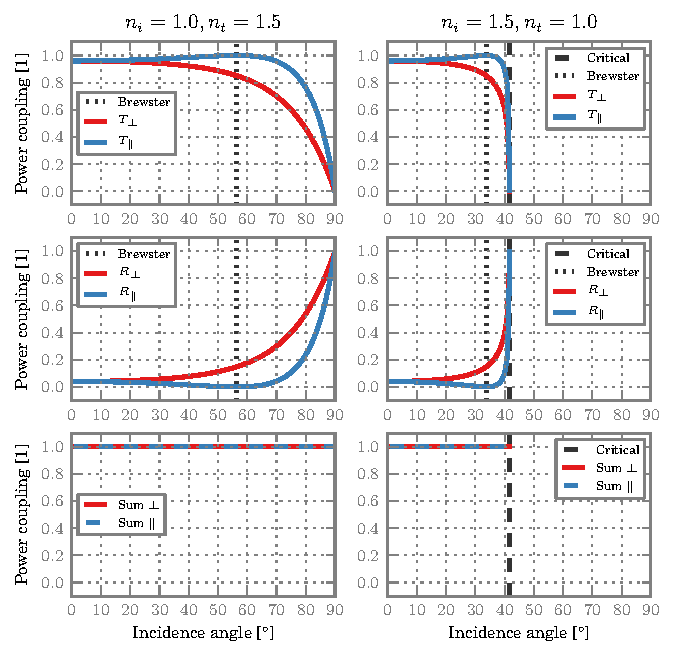
\includegraphics{interface_oblique_verification}
    \caption{Interface oblique, verification}
    \label{fig:interface_oblique_verification}
\end{figure}




%=============================================================================
\clearpage
\subsection{Metallic reflector}
\label{sec:metallic_reflector}
The interface at oblique incidence described in the previous section is limited to dielectrics; or more precisely to materials for which the refractive index is a real number.
Most reflective surfaces inside HIFI are alluminum mirrors.
Alluminum conducts electricity, therefore its refractive index is complex.

When an electromagnetic wave meets a material, its electric field accelerates the electrons of that material.
In return, the accelerating electrons generate an electric field of opposite direction, which creates the reflected wave.
In a conductor, there are free electrons, electrons that are not bound to the atoms of the material.
The free electrons are much more mobile, they can follow the electric field of the incoming wave without being pulled back by their atoms.
As a result, they cancel almost perfectly the electric field of the incoming wave, blocking almost all refraction and generating a quasi-total reflection.

At microwave frequencies, it is customary to consider that metals are perfect reflectors at microwave frequencies.
At normal incidence, the reflection on a metal is very well modeled by a reflection coefficient of~\num{-1}.
Does this still hold at a few terahertz?

As written in~\cref{eq:epsilon_admittivity}, the effect of conductivity~$\sigma'$ of a material is mitigated by the angular frequency~$\omega$:
$\hat{\epsilon} = \epsilon' + i \sigma' / \omega$.
At high frequencies, the electrons cannot accelerate fast enough to cancel the electric field;
as a result, the material becomes more and more transparent, less and less reflective.
Furthermore, the oscillation of the electrons starts lagging behind that of the incoming wave, leading to a noticable phase shift.
Not only does the reflection coefficient get closer to~0, it also gains an imaginary part to represent this phase shift.

The equations of Snell and Fresnel still hold for complex refractive indices
and complex angles of incidence, reflection and refraction.
\Cref{eq:snell_complex} presents Snell's equation with complex angles and indices.
\begin{equation}
    \hat{n}_a \sin \hat{\theta}_a = \hat{n}_b \sin \hat{\theta}_b \label{eq:snell_complex}
\end{equation}

One way to understand complex angles is to consider that rotations are linear transformations.
For example, a rotation of angle~$\hat{\theta}$ around the~$\vect{x}$ axis can be represented by the following matrix
\begin{equation}
    \begin{pmatrix}
        1 & 0 & 0\\
        0 & \cos \hat{\theta} & - \sin \hat{\theta} \\
        0 & \sin \hat{\theta} & \phantom{-}\cos \hat{\theta}
    \end{pmatrix}
\end{equation}
with
\begin{align}
    \cos{\hat{\theta}} &= \frac{\exp(i\hat{\theta}) + \exp(-i\hat{\theta})}{2}
    &
    \sin{\hat{\theta}} &= \frac{\exp(i\hat{\theta}) - \exp(-i\hat{\theta})}{2i}%
    \text{.}
\end{align}
When a complex vector is rotated by a real angle, its components are scaled but the argument of each component is preserved.
When it is rotated by a complex angle, the argument of the components is modified as well.
Complex angles may feel strange at first from a geometrical point of view but are perfectly banal from an algebraic point of view.

One particularity of rotations by complex angles is the following.
Let $\vect{\hat{k}} = \hat{k} \vect{u}$ be a complex vector.
The vector $\vect{u}$ is real and unit and $\hat{k}$ is a complex scalar.
Therefore, the vectors $\vect{k}_r = \Re(\vect{\hat{k}})$ and $\vect{k}_i = \Im(\vect{\hat{k}})$ are collinear.
The rotation by a real angle preserves the collinearity of the real and imaginary parts of a vector.
However, after a rotation by a complex angle, there is no guarantee that the real and imaginary parts of the rotated vector have the same direction.
If $\vect{\hat{k}}$ is a direction of propagation, then the wave is propagating in the direction of the real part of $\vect{\hat{k}}$ but decays in the direction of the imaginary part of $\vect{\hat{k}}$.
When these two directions differ, we say that the wave is inhomogeneous.
Inhomogeneous waves can occur in homogeneous propagation media.
Inhomogeneous waves are not related to anisotropic media either: in an anisotropic medium, there are several real directions of propagation, here there is one real direction and one imaginary direction.

\citeauthor{stratton1941electromagnetic} has worked out the coefficients of reflection and refraction in the case of complex indices in his book \citetitle{stratton1941electromagnetic}~\cite{stratton1941electromagnetic}.
We are not going to rederive them.


%=============================================================================
\clearpage
\subsection{Thin film at normal incidence}
\label{sec:thin_film_at_normal_incidence}


%-----------------------------------------------------------------------------
\subsubsection{Scattering matrix}

Two interfaces separate three regions of space of refractive indices~$n_1$, $n_2$ and~$n_3$ (in most cases, $n_1=n_3$).
Each interface of the film reflects and transmits radiation according to the Fresnel equations for normal incidence~\eqref{eq:fresnel_normal}.
\Cref{fig:thin_film_normal} defines the notations for the reflection and transmission coeffients between the three regions of space.
The propagation between the two interfaces introduces a factor $a$.
\Cref{fig:thin_film_normal_collapsed} is what results of our modeling effort: a single network with two reflections and two transmissions.
\begin{figure}[hbtp]
    \centering
    \input{thin_film_normal.pdf_tex}
    \caption{Thin film at normal incidence.}
    \label{fig:thin_film_normal}
\end{figure}
\begin{figure}[hbtp]
    \centering
    \input{thin_film_normal_collapsed.pdf_tex}
    \caption{Thin film at normal incidence, collapsed.}
    \label{fig:thin_film_normal_collapsed}
\end{figure}

\Crefrange{eq:thin_film_normal_0}{eq:thin_film_normal_2} walk us through the derivation of~$r_{1, 3}$, the reflection coefficient of the thin film seen from the region of refractive index~$n_1$.
\begin{align}
    r_{1,3}
    &= r_{1,2} + t_{1,2}
        \left(
            a r_{2,3} a +
            a r_{2,3} a r_{2,1} a r_{2,3} a +
            \cdots
        \right)
       t_{2,1}
    \label{eq:thin_film_normal_0}
    \\
    r_{1, 3}
    &=
    r_{1, 2} + t_{1, 2} t_{2, 1} a^2r_{2, 3}
        \sum_{i=0}^{\infty} (a^2r_{2,1}r_{2,3})
    \label{eq:thin_film_normal_1}
    \\
    r_{1, 3}
    &=
    r_{1, 2} + t_{1, 2} t_{2, 1} a^2 r_{2, 3}
    \frac{1}{1 - a^2 r_{2, 1} r_{2, 3}}
    \label{eq:thin_film_normal_2}
\end{align}
Likewise, we can derive $r_{3, 1}$, $t_{1, 3}$ and $t_{3, 1}$.
They are given by \crefrange{eq:thin_film_normal_r31}{eq:thin_film_normal_t31},
with \cref{eq:thin_film_normal_r13} being a mere reminder of \cref{eq:thin_film_normal_2}.
\begin{subequations}
    \begin{align}
        r_{1, 3}
        &=
        r_{1, 2} + t_{1, 2} t_{2, 1} a^2 r_{2, 3}
        \frac{1}{1 - a^2 r_{2, 1} r_{2, 3}}
        \label{eq:thin_film_normal_r13}
        \\
        r_{3, 1}
        &=
        r_{3, 2} + t_{3, 2} t_{2, 3} a^2 r_{2, 1}
        \frac{1}{1 - a^2 r_{2, 3} r_{2, 1}}
        \label{eq:thin_film_normal_r31}
        \\
        t_{1, 3}
        &=
        t_{1,2} t_{2,3} a \frac{1}{1 - a^2 r_{2, 3} r_{2, 1}}
        \label{eq:thin_film_normal_t13}
        \\
        t_{3, 1}
        &=
        t_{3,2} t_{2,1} a \frac{1}{1 - a^2 r_{2, 1} r_{2, 3}}
        \label{eq:thin_film_normal_t31}
    \end{align}
\end{subequations}
The parameters $r_{1, 2}$, $t_{1, 2}$, $r_{3, 2}$, $t_{3, 2}$, $r_{2, 1}$, $t_{2, 1}$,
$r_{2, 3}$ and $t_{2, 3}$ are determined by the Fresnel equations for normal incidence~\eqref{eq:fresnel_normal}.
The parameter $a$ is determined by $\exp(-i 2 \pi d n f / c_0)$ according to \cref{eq:net_distance}.
Note that in these four equations, the fraction is the same;
it is sufficient to compute its value once only.



There is one more factor to apply: a compensation for the space taken by the film.
As illustrated in \cref{fig:thin_film_normal_compensation},
the film has a thickness $d_2$ and
its center is located at distances $d_1$ and $d_3$ from other reference points.
The actual length of the medium 1 is not $d_1$ but $d_1 - d_2/2$.
Likewise, the wave travels a distance $d_3 - d_2/2$ in the medium 3.
\begin{figure}[hbtp]
    \centering
    \input{thin_film_normal_compensation.pdf_tex}
    \caption{Thin film at normal incidence, space compensation.}
    \label{fig:thin_film_normal_compensation}
\end{figure}
One way of accounting for this without changing any other network is to add some negative space on each side of the film.
Let $a_1$ and $a_3$ be the effect of these negative spaces.
\Crefrange{eq:negative_space_3}{eq:negative_space_3} apply \cref{eq:net_distance} to the refractive indices $n_1$ and $n_3$ for the negative distance $-d_2/2$.
\begin{subequations}
    \begin{align}
        a_1 &= \exp \Big(-i 2 \pi (-d_2/2) n_1 f / c_0 \Big) \label{eq:negative_space_1}
        \\
        a_3 &= \exp \Big(-i 2 \pi (-d_2/2) n_3 f / c_0 \Big) \label{eq:negative_space_3}
    \end{align}
    \label{eq:negative_space}
\end{subequations}
The reflection on the left side crosses the negative space $a_1$ twice, therefore $r_{1, 3}$ must be multiplied by $a_1^2$.
Likewise, $r_{3, 1}$ must be multiplied by $a_3^2$.
Both transmissions $t_{1, 3}$ and $t_{3, 1}$ go through $a_1$ and $a_3$, therefore they must be multiplied by $a_1 a_3$.
This is summarized with \crefrange{eq:thin_film_normal_compensated_r13}{eq:thin_film_normal_compensated_t31}.
\begin{subequations}
    \begin{align}
        r'_{1, 3} &= a_1^2   \, r_{1, 3} \label{eq:thin_film_normal_compensated_r13} \\
        r'_{3, 1} &= a_3^2   \, r_{3, 1} \label{eq:thin_film_normal_compensated_r31} \\
        t'_{1, 3} &= a_1 a_3 \, t_{1, 3} \label{eq:thin_film_normal_compensated_t13} \\
        t'_{3, 1} &= a_1 a_3 \, t_{3, 1} \label{eq:thin_film_normal_compensated_t31}
    \end{align}
    \label{eq:thin_film_normal_compensated}
\end{subequations}

From there, building the scattering matrix of the thin film is straightforward.
If we name $I_3$ the 3--by--3 identity matrix,
then the Jones matrices  \crefrange{eq:thin_film_normal_s11}{eq:thin_film_normal_s22}
are the elements of the scattering matrix.
\begin{subequations}
    \begin{align}
        S_{1, 1} &= r'_{1, 3} I_3 \label{eq:thin_film_normal_s11} \\
        S_{1, 2} &= t'_{3, 1} I_3 \label{eq:thin_film_normal_s12} \\
        S_{2, 1} &= t'_{1, 3} I_3 \label{eq:thin_film_normal_s21} \\
        S_{2, 2} &= r'_{3, 1} I_3 \label{eq:thin_film_normal_s22}
    \end{align}
    \label{eq:thin_film_normal_sij}
\end{subequations}
If necessary, each of these Jones matrices can be adapted to account for the orientation of the thin film;
see~\vref{sec:rotating_jones_matrices}.

%-----------------------------------------------------------------------------
\subsubsection{Verification}
We have derived a model that treats a thin film as a single two-port network.
It should yield the same results as a system of three networks
(interface--space--interface).
In this section, we verify this numerically.

\Cref{fig:thin_film_normal_verification_principle} defines the distances and refractive indices used in this section.
It also illustrates the two systems that we wish to compare:
\begin{itemize}
    \item one system made of three networks (two spaces, one thin film), that we call ``thin film model'';
    \item one system made of five networks (three spaces and two interfaces), that we call ``interfaces model''.
\end{itemize}
\begin{figure}[hbtp]
    \centering
    \input{thin_film_normal_verification_principle.pdf_tex}
    \caption{Thin film at normal incidence, verification, principle.}
    \label{fig:thin_film_normal_verification_principle}
\end{figure}

\Cref{fig:thin_film_normal_verification} presents the result of both models for
$n_1=1.00$, $n_2=1.75$, $n_3=1.50$,
$d_1=\SI{1}{\meter}$, $d_2=\SI{10}{\micro\meter}$ and $d_3=\SI{1}{\meter}$.
The source is on the leftmost port.
The ``Reflected'' plot corresponds to the output of that leftmost port.
The ``Transmitted'' plot corresponds to the output of the rightmost port.
\begin{figure}[hbtp]
    \centering
    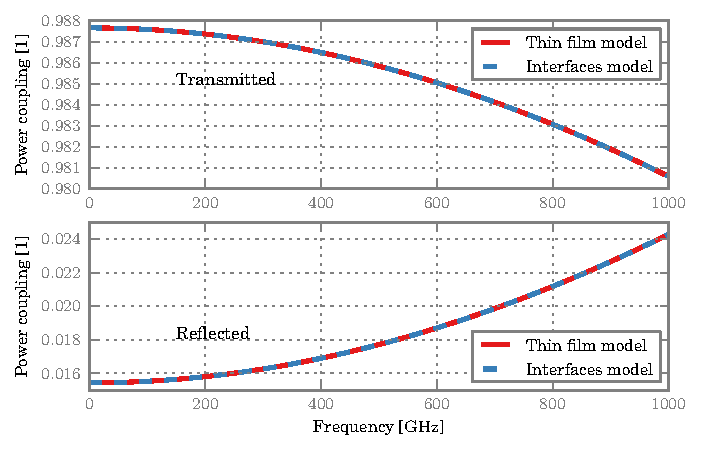
\includegraphics{thin_film_normal_verification.pdf}
    \caption{Thin film at normal incidence, verification.}
    \label{fig:thin_film_normal_verification}
\end{figure}

Both models agree within numerical noise.
The advantage of the thin film model over the other is that a thin film is represented by a single network.
This is easier for the programmer and faster for the computer.

The curvature of the power coupling displayed in \cref{fig:thin_film_normal_verification} comes from standing waves inside the thin film.
\Cref{eq:cavity_period} predicts a period of $F = c_0 / (2 n_2 d_2) \approx \SI{9993}{\tera\hertz}$.
Thin cavities (here \SI{10}{\micro\meter}) create standing wave patterns with very large periods.



%=============================================================================
\subsection{Thin film at oblique incidence}
\label{sec:thin_film_at_oblique_incidence}

A thin film at oblique incidence forms a four-port network.
\Cref{fig:thin_film_oblique} defines the geometry and the port-numbering that we use.
\begin{figure}[hbtp]
    \centering
    \missingfigure{Thin film oblique}
    \caption{Thin film at oblique incidence}
    \label{fig:thin_film_oblique}
\end{figure}

When deriving the scattering matrix of a thin film at normal incidence in \cref{sec:thin_film_at_normal_incidence}, we allowed for three refractive indices: one for the film itself and one for each propagation medium on each side of the film.
This was a generalization that came at barely no cost because the geometry was simple.
In the case of a thin film at oblique incidence, we assume that the propagation medium on each side of the thin film has the same refractive index.
This is, after all, the most common case;
for example, a beam splitter placed in vacuum has vacuum on both sides.
If that constraint is too strong, it is always possible to model that thin film with three networks by using two interfaces and a distance (see sections~\ref{sec:generic_networks_distance} and \ref{sec:interface_at_oblique_incidence}).

%-----------------------------------------------------------------------------
\subsubsection{Geometry}
\label{sec:thin_film_geometry}
We need to determine the angle of incidence, the parallel and perpendicular decomposition matrices and the various rotation matrices.

It is assumed that we know the orientation of the thin film via its normal $n$ and the direction of propagation $k_1$ of the wave incident to the port 1.

From $n$ and $k_1$, we can apply \cref{eq:angle_from_dot_product} to compute the angle of incidence~$\theta_a$.
We get the refracted angle~$\theta_b$ from $\theta_a$ with \cref{eq:snell_thetab}.

We use \cref{eq:normal_to_plane_of_incidence} to retreive the normal to the plane-of-incidence $u$.

From the normal $u$ to the plane-of-incidence
and \cref{eq:para_perp_decomposition_matrix},
we determine the parallel and perpendicular projection matrices,
$M_\parallel$ and $M_\perp$.

From $u$ and
equations~\eqref{eq:quaternion_rotation_around_axis}
and \eqref{eq:quaternion_to_rotation_matrix}, we can compute the rotation matrices to apply to the Jones matrices and the direction of propagation.
The angles that we need are listed in \cref{eq:thin_film_angles}.
\begin{equation}
    \begin{aligned}
        \theta_{1 \leftarrow 2} &= 2 \theta_a
        &
        \theta_{2 \leftarrow 1} &= -2 \theta_a
        \\
        \theta_{3 \leftarrow 4} &= 2 \theta_a
        &
        \theta_{4 \leftarrow 3} &= -2 \theta_a
        \\
        \theta_{4 \leftarrow 1} &= -2 \theta_a
    \end{aligned}
    \label{eq:thin_film_angles}
\end{equation}
These angles $\theta_{i \leftarrow j}$ have corresponding rotation matrices $R^{i \leftarrow j}$.
We can already determine the directions of propagation of the waves exiting the thin film with \cref{eq:thin_film_propagation_rotation_ki}.
\begin{subequations}
    \begin{align}
        k_2 &= -R^{2 \leftarrow 1} k_1
        \label{eq:thin_film_propagation_rotation_k2}\\
        k_3 &= k_1
        \label{eq:thin_film_propagation_rotation_k3}\\
        k_4 &= R^{4 \leftarrow 1} k_1
        \label{eq:thin_film_propagation_rotation_k4}
    \end{align}
    \label{eq:thin_film_propagation_rotation_ki}
\end{subequations}

%-----------------------------------------------------------------------------
\subsubsection{Reflection and transmission coefficients}
In the previous section (\cref{sec:thin_film_geometry}) we have determined the decomposition and rotation matrices that are needed to compute the reflection and refraction coefficients of a thin film at oblique incidence.
We also have the angle of incidence and the refracted angle.

We want to apply the Fresnel equations for oblique incidence \eqref{eq:fresnel_oblique} twice:
once for entering the thin film, and once for leaving it.
\begin{itemize}
    \item 
$r_{\parallel a}$, $r_{\perp a}$, $t_{\parallel a}$ and $t_{\perp a}$ correspond to entering the film.
They are derived from \cref{eq:fresnel_oblique} with
$\theta_i = \theta_a$, $\theta_t = \theta_b$,
$n_i = n_a$ and $n_t = n_b$.
    \item
$r_{\parallel b}$, $r_{\perp b}$, $t_{\parallel b}$ and $t_{\perp b}$ correspond to exiting the film.
They are derived from \cref{eq:fresnel_oblique} with
$\theta_i = \theta_b$, $\theta_t = \theta_a$,
$n_i = n_b$ and $n_t = n_a$.
\end{itemize}

The pathlength $l_b$ inside the film is not equal to the thickness $d$ of the thin film because $\theta_b \ne 0$, as described by \cref{eq:thin_film_oblique_pathlength}.
\begin{equation}
    l_b = \frac{d}{\cos \theta_b}
    \label{eq:thin_film_oblique_pathlength}
\end{equation}
To this distance $l_b$ corresponds a gain $a_b$ that we derive from \cref{eq:net_distance}.
Its expression is given for $l_b$ in \cref{eq:thin_film_distance}.
\begin{equation}
    a_b = \exp(-2i \pi l_b n_b f / c_0)
    \label{eq:thin_film_distance}
\end{equation}
This pathlength $l_b$ must be compensated for.
Indeed, the pathlength $l_b$ inside the film replaces a pathlength $l_a$ in the material $n_a$.
\begin{equation}
    l_a = \frac{d}{\cos \theta_a}
    \label{eq:thin_film_oblique_pathlength_compensation}
\end{equation}
\begin{equation}
    a_a = \exp(-2i \pi (-l_a) n_a f / c_0)
    \label{eq:thin_film_distance_compensation}
\end{equation}

What follows is similar to what we did for the thin film at normal incidence.
One difference is that do it twice, one for the parallel parameters and one for the perpendicular parameters.
Another difference is that we have two and not three refractive indices, which gives a few simplifications.
\begin{subequations}
    \begin{align}
        t_\parallel
        &=
        a_a \,
        t_{\parallel a} \, t_{\parallel b} \, a_b
        \frac{1}{
            1 - (r_{\parallel b} \, a_b)^2
        }
        \\
        t_\perp
        &=
        a_a \,
        t_{\perp a} \, t_{\perp b} \, a_b
        \frac{1}{
            1 - (r_{\perp b} \, a_b)^2
        }
        \\
        r_\parallel
        &=
        a_a \,
        r_{\parallel a} + r_{\parallel b} \, a_b \, t_\parallel
        \\
        r_\perp
        &=
        a_a \,
        r_{\perp a} + r_{\perp b} \, a_b \, t_\perp
    \end{align}
\end{subequations}

\subsubsection{Scattering matrix}
Because we use one refractive index only outside the film, the transmitted waves are not rotated.
\begin{equation}
    S_{1, 3} =
    S_{2, 4} =
    S_{3, 1} =
    S_{4, 2} =
    t_\parallel M_\parallel
    +
    t_\perp M_\perp
    \label{eq:thin_film_s_t}
\end{equation}

The reflections, however, require some rotations.
\begin{subequations}
    \begin{align}
        S_{1, 2} = R^{1 \leftarrow 2} (r_\parallel M_\parallel + r_\perp M_\perp) \\
        S_{2, 1} = R^{2 \leftarrow 1} (r_\parallel M_\parallel + r_\perp M_\perp) \\
        S_{3, 4} = R^{3 \leftarrow 4} (r_\parallel M_\parallel + r_\perp M_\perp) \\
        S_{4, 3} = R^{4 \leftarrow 3} (r_\parallel M_\parallel + r_\perp M_\perp)
    \end{align}
    \label{eq:thin_film_s_r}
\end{subequations}

Finally, many paths are forbidden.
\begin{equation}
    S_{1, 1} = S_{1, 4} = S_{2, 2} = S_{2, 3} =
    S_{3, 2} = S_{3, 3} = S_{4, 1} = S_{4, 4} = 
    \begin{pmatrix}
        0&0&0\\0&0&0\\0&0&0
    \end{pmatrix}
    \label{eq:thin_film_s_zero}
\end{equation}

\Crefrange{eq:thin_film_s_t}{eq:thin_film_s_zero} define the scattering parameters of the 4--by--4 scattering matrix of a thin film at oblique incidence.


\subsubsection{Verification}
Our model for a thin film at oblique incidence should provide exactly the same result as two interfaces and a distance.
The goal of the thin film model is to provide convenience, not introduce new physics.
\Cref{fig:thin_film_oblique_verification} illustrates a comparison between these two ways of modeling a thin film.
The angle of incidence is~\SI{45}{\degree}.
The film is~\SI{10}{\micro\meter} thick.
The refractive indices are 1.0 outside the film and 1.5 in the film.
The thickness of the film creates a cavity and therefore a standing wave.
This standing wave is responsable for the frequency-dependance of the reflected and transmitted power seen on \cref{fig:thin_film_oblique_verification}.

\begin{figure}[hbtp]
    \centering
    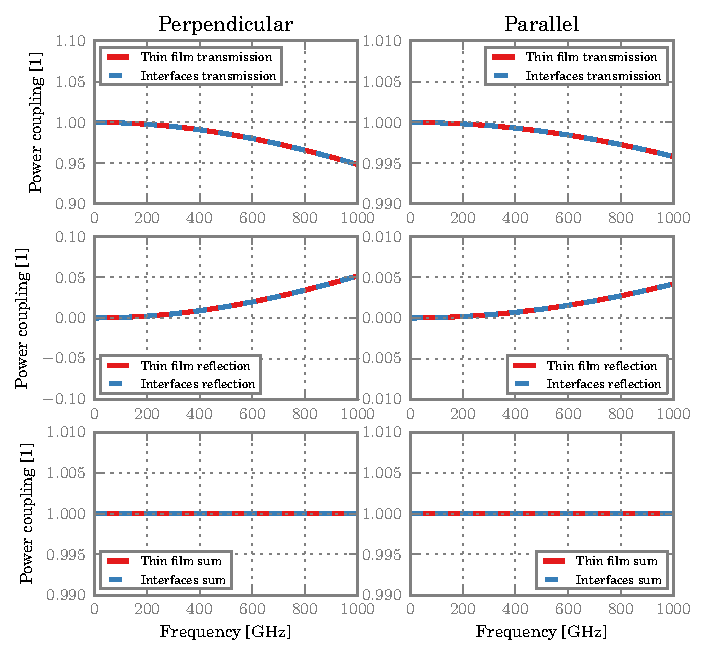
\includegraphics{thin_film_oblique_verification}
    \caption{Thin film at oblique incidence, verification}
    \label{fig:thin_film_oblique_verification}
\end{figure}

The top row of \cref{fig:thin_film_oblique_verification} shows the transmitted power, the middle row shows the reflected power, and the bottom row shows the sum of the two.
That last row shows that energy is conserved: the power that is not transmitted is reflected.

The left column shows the transmitted, reflected and total power coupling for the perpendicular polarization.
The right column corresponds to the parallel polarization.
Note that the vertical-axes differ for the two polarizations: the standing wave has an effect about ten times stronger on the perpendicular polarization.

Finally, each plot shows two overlapped curves.
The red curve corresponds to the model derived in this section with which the thin film is seen as a single network.
The blue curve corresponds to a model made of two interfaces and a distance.

As expected, both models agree within numerical noise.
This agreement does not only happen in power, but also in field.
The phasor predicted by both methods agree within $10^{-10}$: the magnitude of the difference of the phasors is smaller than $10^{-10}$ for frequencies of the order of \SI{1}{\tera\hertz}.  \todo{Should I put a pic?}



%=============================================================================
\subsection{Wire grid polarizer}
\todo{Check k omega convention}
In their paper from \citeyear{houde_2001} \citetitle{houde_2001}, \textcite{houde_2001} present a set of equations that approximate the electric field at any point near a wire grid polarizer.
The incident wave is assumed plane, the surrounding propagation medium is assumed homogeneous and isotropic, and the wires are assumed to be free floating (no dielectric substrate) and to have a cylindrical section.

\subsubsection{Geometry}
The article of \citeauthor{houde_2001} \cite{houde_2001} defines the following rest reference frame for the grid: wires in the $\vect{x}\vect{y}$ plane, wires along $\vect{x}$.
Its normal, at rest, is therefore the $\vect{z}$ axis.

If $R$ is the rotation matrix that move the grid from its rest attitude to its useful attitude, then the normal of the grid is $\vect{n}=R \vect{z}$.

The grid is a four port network.
$\vect{k}_1$,  is the direction of propagation of the wave indident to the port 1.
We can derive the direction of propagation of the wave incident to the three other ports easily.
The law of reflection states that $\vect{k}_1$, $\vect{k}_2$ and $\vect{n}$ are coplanar and that the directed angle between $\vect{k}_1$ and $\vect{n}$ equals that between $\vect{n}$ and $\vect{k}_2$.
Therefore, one way of deriving $\vect{k}_2$ is to rotate $\vect{k}_1$ by \SI{180}{\degree} around $\vect{n}$.
Then, $\vect{k}_3=-\vect{k}_1$ and $\vect{k}_4=-\vect{k_2}$.

\subsubsection{Reflection and transmission coefficients}
The set of equations that interest us here are the equations numbered 23 to 35, 62 and 63 in the article of \citeauthor{houde_2001} \cite{houde_2001}, which we copied here for convenience.
The first two equations, \eqref{eq:grid_current_linear} and \eqref{eq:grid_current_circular}, describe the electric current in the wires.
$K^x$ corresponds to a linear current and $K^\theta$ to a circular current.
In the first case, electrons move along the length of the wire; in the other, they rotate around the axis of the wire.
\begin{align}
    K^x &= \frac{E_0}{F} \cdot \alpha' \frac{N_x}{\Delta_x}
    \label{eq:grid_current_linear}
    \\
    K^\theta &= (-j) \frac{E_0}{F} \cdot (\gamma' \beta - \beta' \gamma) \frac{N_\theta}{\Delta_\theta}
    \label{eq:grid_current_circular}
\end{align}
with
\begin{align}
    N_x
    &=
    1 - j \frac{Z_s}{Z_0} \frac{ka}{2}
    \\
    \Delta_x
    &=
    (1 - \alpha^2) S_1 - j \frac{Z_s}{Z_0} \sqrt{1 - \alpha^2}H_1^{(2)} (k'a)
    \\
    N_\theta
    &=
    1 + j \frac{Z_s}{Z_0} \frac{2}{ka}
    \\
    \Delta_\theta
    &=
    \sqrt{1 - \alpha^2} H_1^{(2)} (k'a) + j \frac{Z_s}{Z_0} (1 - \alpha^2) S_1
\end{align}
and
\begin{equation}
    S_1 = H_0^{(2)} (k'a) + 2
    \sum_{n=1}^\infty
    H_0^{(2)}(k'nd) \cos (k \beta nd)
    \text{.}
    \label{eq:infinite_hankel}
\end{equation}
The following equations use the previous definitions.
They describe the reflected and transmitted fields in three dimensions for a grid in the $xy$-plane, wires along~$x$.
\begin{align}
    R^x
    &=
    -\frac{F}{E_0}
    \frac{\lambda}{\pi d}
    \frac{1 - \alpha^2}{\gamma} K^x
    \label{eq:houde_Rx}
    \\
    R^y
    &=
    \phantom{-}
    \frac{F}{E_0}
    \frac{\lambda}{\pi d}
    \left[
        \frac{\alpha \beta}{\gamma} K^x
        -
        j \frac{ka}{2} K^\theta
    \right]
    \\
    R^z
    &=
    -\frac{F}{E_0}
    \frac{\lambda}{\pi d}
    \left[
       \alpha K^x
       +
       j \frac{\beta}{\gamma} \frac{ka}{2} K^\theta
    \right]
    \\
    T^x &= \alpha' + R^x
    \\
    T^y
    &=
    \beta' +
    \frac{F}{E_0}
    \frac{\lambda}{\pi d}
    \left[
        \frac{\alpha \beta}{\gamma} K^x + j \frac{ka}{2} K^\theta
    \right]
    \\
    T^z
    &=
    \gamma' +
    \frac{F}{E_0}
    \frac{\lambda}{\pi d}
    \left[
        \alpha K^x - j \frac{\beta}{\gamma} \frac{ka}{2} K^\theta
    \right]
\end{align}
Note that Houde calls these $R$ and $T$ ``reflection'' and ``transmission coefficient'', something they are not quite since they contain $\alpha'$, $\beta'$ and $\gamma'$, corresponding to the amplitude of the incoming electric field in the three dimensions.
These amplitudes have to be factored out if we want to really speak about reflection or transmission coefficients.

When implementing these equations, some simplifications are obvious.
For example, $\frac{E_0}{F}$ inside $K^x$ and $K^\theta$ cancels $\frac{F}{E_0}$ in $R$ and $T$;
the complex unit $j$ within $K^\theta$ combines with $j$ in $R$ and $T$ to become -1.

In these equations, $\alpha'$, $\beta'$ and $\gamma'$ are the three components of the direction of the incident electric field, satisfying $\alpha'^2 + \beta'^2 + \gamma'^2 = 1$.
That condition seems to apply only to real numbers, restricting the use of this grid model to waves that are linearly polarized (their three components are in phase).
However, there is no such limitation in the model.
Indeed, the authors define the incident electric field as $(e_x, e_y, e_z) = E_0(\alpha', \beta', \gamma')$.
The amplitude $E_0$ can be complex and it seems that its phase has to be shared among the three components.
However, when we rewrite the equations to fit in a matrix, we will notice that the real parameters are not $\alpha'$, $\beta'$, $\gamma'$ and $E_0$, but $e_x$, $e_y$ and $e_z$ directly, which are all independant.
In that case, each of them is free to have its own phase and the model also applies to elliptically polarized waves.


In order to rewrite these equations in a matrix form that depends on $e_x$, $e_y$ and $e_z$, one needs to split each coefficient of transmission and reflection into three, like this:
\begin{equation}
    e_{rx} = R^{xx} e_x + R^{xy} e_y + R^{xz} e_z
\end{equation}
so that we can write
\begin{align}
    e_r &= R e_i \\
    e_r &=
    \begin{pmatrix}
        R_{xx} & R_{xy} & R_{xz} \\
        R_{yx} & R_{yy} & R_{yz} \\
        R_{zx} & R_{zy} & R_{zz}
    \end{pmatrix}
    e_i
\end{align}
for the reflection $R$ and a similar equation for the transmission $e_t = T e_i$.
I start with $R_x$ defined in \cref{eq:houde_Rx} to get $R_{xx}$, $R_{xy}$ and $R_{xz}$.
\begin{align*}
    e_{rx} &= R^x E_0
    \\
           &= -\frac{F}{E_0}
              \frac{\lambda}{\pi d}
              \frac{1-\alpha^2}{\gamma}
              K^x
              E_0
    \\
           &= -\cancel{\frac{F}{E_0}}
              \frac{\lambda}{\pi d}
              \frac{1-\alpha^2}{\gamma}
              \cancel{\frac{E_0}{F}}
              \frac{N_x}{\Delta_x}
              \underbrace{
                  \alpha'
                  E_0
              }_{e_{ix}}
    \\
           &= -\frac{\lambda}{\pi d}
              \frac{1-\alpha^2}{\gamma}
              \frac{N_x}{\Delta_x}
              e_{ix}
\end{align*}
By identification, we find these values for $R_{xx}$, $R_{xy}$ and $R_{xz}$.
\begin{equation}
    \left\lbrace
    \begin{aligned}
        R_{xx} &= -\frac{\lambda}{\pi d}
                  \frac{N_x}{\Delta_x}
                  \frac{1-\alpha^2}{\gamma}
        \\
        R_{xy} &= 0
        \\
        R_{xz} &= 0
    \end{aligned}
    \right.
\end{equation}
Let us continue with $R_y$.
\begin{align*}
    e_{ry}
    &= R^y E_0
    \\
    &= \frac{F}{E_0}
       \frac{\lambda}{\pi d}
       \left[
           \frac{\alpha \beta}{\gamma}
           K^x
           -
           j
           \frac{ka}{2}
           K^\theta           
       \right]
       E_0
    \\
    &= \cancel{\frac{F}{E_0}}
       \frac{\lambda}{\pi d}
       \left[
           \frac{\alpha \beta}{\gamma}
           \cancel{\frac{E_0}{F}}
           \frac{N_x}{\Delta_x}
           \alpha'
           -
           j
           \frac{ka}{2}
           (-j)
           \cancel{\frac{E_0}{F}}
           \frac{N_\theta}{\Delta_\theta}
           (\gamma' \beta - \beta' \gamma)           
       \right]
       E_0
    \\
    &= \frac{\lambda}{\pi d}
       \left[
           \frac{\alpha \beta}{\gamma}
           \frac{N_x}{\Delta_x}
           \alpha'
           +
           \frac{ka}{2}
           \frac{N_\theta}{\Delta_\theta}
           \gamma
           \beta'
           -
           \frac{ka}{2}
           \frac{N_\theta}{\Delta_\theta}
           \beta
           \gamma'
       \right]
       E_0
    \\
    &= \frac{\lambda}{\pi d}
       \frac{\alpha \beta}{\gamma}
       \frac{N_x}{\Delta_x}
       \underbrace{E_0 \alpha'}_{e_{ix}}
       +
       \frac{\lambda}{\pi d}
       \frac{ka}{2}
       \frac{N_\theta}{\Delta_\theta}
       \gamma
       \underbrace{E_0 \beta'}_{e_{iy}}
       -
       \frac{\lambda}{\pi d}
       \frac{ka}{2}
       \frac{N_\theta}{\Delta_\theta}
       \beta
       \underbrace{E_0 \gamma'}_{e_{iz}}
\end{align*}
\begin{equation}
    \left\lbrace
    \begin{aligned}
        R_{yx}
        &=
        \phantom{-}
        \frac{\lambda}{\pi d}
        \frac{N_x}{\Delta_x}
        \frac{\alpha \beta}{\gamma}
        \\
        R_{yy}
        &=
        \phantom{-}
        \frac{\lambda}{\pi d}
        \frac{N_\theta}{\Delta_\theta}
        \frac{ka}{2}
        \gamma
        \\
        R_{yz}
        &=
        -
        \frac{\lambda}{\pi d}
        \frac{N_\theta}{\Delta_\theta}
        \frac{ka}{2}
        \beta
    \end{aligned}
    \right.
\end{equation}
Same thing for $R_z$.
\begin{align*}
    e_{rz} &= R^z E_0
    \\
    &=
    -
    \frac{F}{E_0}
    \frac{\lambda}{\pi d}
    \left[
        \alpha K^x
        +
        j
        \frac{\beta}{\gamma}
        \frac{ka}{2}
        k^\theta
    \right]
    E_0
    \\
    &=
    -
    \cancel{\frac{F}{E_0}}
    \frac{\lambda}{\pi d}
    \left[
        \alpha
        \cancel{\frac{E_0}{F}}
        \frac{N_x}{\Delta_x}
        \alpha'
        +
        j
        \frac{\beta}{\gamma}
        \frac{ka}{2}
        (-j)
        \cancel{\frac{E_0}{F}}
        (\gamma' \beta - \beta' \gamma)
        \frac{N_\theta}{\Delta_\theta}
    \right]
    E_0
    \\
    &=
    -
    \frac{\lambda}{\pi d}
    \alpha
    \frac{N_x}{\Delta_x}
    \underbrace{E_0 \alpha'}_{e_{ix}}
    +
    \frac{\lambda}{\pi d}
    \frac{\beta}{\gamma}
    \frac{ka}{2}
    \frac{N_\theta}{\Delta_\theta}
    \gamma
    \underbrace{E_0 \beta'}_{e_{iy}}
    -
    \frac{\lambda}{\pi d}
    \frac{\beta}{\gamma}
    \frac{ka}{2}
    \frac{N_\theta}{\Delta_\theta}
    \beta
    \underbrace{E_0 \gamma'}_{e_{iz}}
\end{align*}
\begin{equation}
    \left\lbrace
    \begin{aligned}
        R_{zx}
        &=
        -
        \frac{\lambda}{\pi d}
        \frac{N_x}{\Delta_x}
        \alpha
        \\
        R_{zy}
        &=
        \phantom{-}
        \frac{\lambda}{\pi d}
        \frac{N_\theta}{\Delta_\theta}
        \frac{ka}{2}
        \beta
        \\
        R_{zz}
        &=
        -
        \frac{\lambda}{\pi d}
        \frac{N_\theta}{\Delta_\theta}
        \frac{ka}{2}
        \frac{\beta^2}{\gamma}
    \end{aligned}
    \right.
\end{equation}
We have the reflection matrix.
Now, we compute the transmission matrix.
\begin{align*}
    e_{tx} &= T^x E_0
    \\
    &= (\alpha' + R^x) E_0
    \\
    &= \underbrace{\alpha' E_0}_{e_{ix}}
       -
       \frac{\lambda}{\pi d}
       \frac{1 - \alpha^2}{\gamma}
       \frac{N_x}{\Delta_x}
       \underbrace{\alpha' E_0}_{e_{ix}}
    \\
    &= \left(
           1
           -
           \frac{\lambda}{\pi d}
           \frac{1 - \alpha^2}{\gamma}
           \frac{N_x}{\Delta_x}
       \right)
       e_{ix}
\end{align*}
\begin{equation}
    \left\lbrace
    \begin{aligned}
        T_{xx}
        &= 1
           -
           \frac{\lambda}{\pi d}
           \frac{N_x}{\Delta_x}
           \frac{1 - \alpha^2}{\gamma}
        \\
        T_{xy} &= 0
        \\
        T_{xz} &= 0
    \end{aligned}
    \right.
\end{equation}

\begin{align*}
    e_{ty} &= T^y E_0
    \\
    &=
    \left(
        \beta'
        +
        \frac{F}{E_0}
        \frac{\lambda}{\pi d}
        \left[
            \frac{\alpha \beta}{\gamma}
            K^x
            +
            j
            \frac{ka}{2}
            K^\theta
        \right]
    \right)
    E_0
    \\
    &=
    \left(
        \beta'
        +
        \cancel{\frac{F}{E_0}}
        \frac{\lambda}{\pi d}
        \left[
            \frac{\alpha \beta}{\gamma}
            \cancel{\frac{E_0}{F}}
            \frac{N_x}{\Delta_x}
            \alpha'
            +
            j
            \frac{ka}{2}
            (-j)
            \cancel{\frac{E_0}{F}}
            \frac{N_\theta}{\Delta_\theta}
            (\gamma' \beta - \beta' \gamma)
        \right]
    \right)
    E_0
    \\
    &=
    \left(
        \beta'
        +
        \frac{\lambda}{\pi d}
        \frac{\alpha \beta}{\gamma}
        \frac{N_x}{\Delta_x}
        \alpha'
        -
        \frac{\lambda}{\pi d}
        \frac{ka}{2}
        \frac{N_\theta}{\Delta_\theta}
        \gamma
        \beta'
        +
        \frac{\lambda}{\pi d}
        \frac{ka}{2}
        \frac{N_\theta}{\Delta_\theta}
        \beta
        \gamma'
    \right)
    E_0
    \\
    &=
    \frac{\lambda}{\pi d}
    \frac{\alpha \beta}{\gamma}
    \frac{N_x}{\Delta_x}
    \underbrace{E_0 \alpha'}_{e_{ix}}
    +
    \left(
        1
        -
        \frac{\lambda}{\pi d}
        \frac{ka}{2}
        \frac{N_\theta}{\Delta_\theta}
        \gamma
    \right)
    \underbrace{E_0 \beta'}_{e_{iy}}
    +
    \frac{\lambda}{\pi d}
    \frac{ka}{2}
    \frac{N_\theta}{\Delta_\theta}
    \beta
    \underbrace{E_0 \gamma'}_{e_{iz}}
\end{align*}
\begin{equation}
    \left\lbrace
    \begin{aligned}
        T_{yx}
        &= \frac{\lambda}{\pi d}
           \frac{N_x}{\Delta_x}
           \frac{\alpha \beta}{\gamma}
        \\
        T_{yy}
        &= 1
           -
           \frac{\lambda}{\pi d}
           \frac{N_\theta}{\Delta_\theta}
           \frac{ka}{2}
           \gamma
        \\
        T_{yz}
        &= \frac{\lambda}{\pi d}
           \frac{N_\theta}{\Delta_\theta}
           \frac{ka}{2}
           \beta
    \end{aligned}
    \right.
\end{equation}

\begin{align*}
    e_{tz} &= T^z E_0
    \\
    &=
    \left(
        \gamma' +
        \frac{F}{E_0}
        \frac{\lambda}{\pi d}
        \left[
            \alpha K^x - j \frac{\beta}{\gamma} \frac{ka}{2} K^\theta
        \right]
    \right)
    E_0
    \\
    &=
    \left(
        \gamma' +
        \cancel{\frac{F}{E_0}}
        \frac{\lambda}{\pi d}
        \left[
            \alpha
            \cancel{\frac{E_0}{F_0}}
            \frac{N_x}{\Delta_x}
            \alpha'
            -
            j
            \frac{\beta}{\gamma}
            \frac{ka}{2}
            (-j)
            \cancel{\frac{E_0}{F}}
            \frac{N_\theta}{\Delta_\theta}
            (\gamma' \beta - \beta' \gamma)
        \right]
    \right)
    E_0
    \\
    &=
    \left(
        \gamma' +
        \frac{\lambda}{\pi d}
        \left[
            \alpha
            \frac{N_x}{\Delta_x}
            \alpha'
            +
            \frac{\beta}{\gamma}
            \frac{ka}{2}
            \frac{N_\theta}{\Delta_\theta}
            \gamma
            \beta'
            -
            \frac{\beta}{\gamma}
            \frac{ka}{2}
            \frac{N_\theta}{\Delta_\theta}
            \beta
            \gamma'
        \right]
    \right)
    E_0
    \\
    &=
    \frac{\lambda}{\pi d}
    \alpha
    \frac{N_x}{\Delta_x}
    \underbrace{E_0 \alpha'}_{e_{ix}}
    +
    \frac{\lambda}{\pi d}
    \frac{\beta}{\gamma}
    \frac{ka}{2}
    \frac{N_\theta}{\Delta_\theta}
    \gamma
    \underbrace{E_0 \beta'}_{e_{iy}}
    +
    \left(
        1
        -
        \frac{\lambda}{\pi d}
        \frac{\beta}{\gamma}
        \frac{ka}{2}
        \frac{N_\theta}{\Delta_\theta}
        \beta
    \right)
    \underbrace{E_0 \gamma'}_{e_{iz}}
\end{align*}
\begin{equation}
    \left\lbrace
    \begin{aligned}
        T_{zx}
        &= \frac{\lambda}{\pi d}
           \frac{N_x}{\Delta_x}
           \alpha
        \\
        T_{zy}
        &= \frac{\lambda}{\pi d}
           \frac{N_\theta}{\Delta_\theta}
           \frac{ka}{2}
           \frac{\beta}{\gamma}
           \gamma
        \\
        T_{zz}
        &= 1
           -
           \frac{\lambda}{\pi d}
           \frac{N_\theta}{\Delta_\theta}
           \frac{ka}{2}
           \frac{\beta}{\gamma}
           \beta
    \end{aligned}
    \right.
\end{equation}

Another simplification:
\begin{equation}
    k = 2\pi / \lambda
    \quad \Rightarrow \quad
    \frac{\lambda}{\pi d} \frac{ka}{2}
    =
    \frac{\lambda}{\pi d} \frac{2\pi a}{2\lambda}
    =
    \frac{a}{d}
\end{equation}

\begin{equation}
    R =
    \begin{pmatrix}
        -\frac{\lambda}{\pi d}
        \frac{N_x}{\Delta_x}
        \frac{1 - \alpha^2}{\gamma}
        &
        0
        &
        0
        \\
        \frac{\lambda}{\pi d}
        \frac{N_x}{\Delta_x}
        \frac{\alpha \beta}{\gamma}
        &
        \frac{\lambda}{\pi d}
        \frac{N_\theta}{\Delta_\theta}
        \frac{ka}{2}
        \gamma
        &
        -
        \frac{a}{d}
        \frac{N_\theta}{\Delta_\theta}
        \beta
        \\
        -
        \frac{\lambda}{\pi d}
        \frac{N_x}{\Delta_x}
        \alpha
        &
        \frac{a}{d}
        \frac{N_\theta}{\Delta_\theta}
        \beta
        &
        -
        \frac{a}{d}
        \frac{N_\theta}{\Delta_\theta}
        \frac{\beta^2}{\gamma}
    \end{pmatrix}
\end{equation}
\begin{equation}
    T =
    \begin{pmatrix}
        1 -
        \frac{\lambda}{\pi d}
        \frac{N_x}{\Delta_x}
        \frac{1 - \alpha^2}{\gamma}
        &
        0
        &
        0
        \\
        \frac{\lambda}{\pi d}
        \frac{N_x}{\Delta_x}
        \frac{\alpha \beta}{\gamma}
        &
        1 -
        \frac{a}{d}
        \frac{N_\theta}{\Delta_\theta}
        \gamma
        &
        \frac{a}{d}
        \frac{N_\theta}{\Delta_\theta}
        \beta
        \\
        \frac{\lambda}{\pi d}
        \frac{N_x}{\Delta_x}
        \alpha
        &
        \frac{a}{d}
        \frac{N_\theta}{\Delta_\theta}
        \beta
        &
        1 -
        \frac{a}{d}
        \frac{N_\theta}{\Delta_\theta}
        \frac{\beta^2}{\gamma}
    \end{pmatrix}
\end{equation}
These reflection and transmission matrices are Jones matrices.
The parameters are the radius $a$ of the wires,
the distance $d$ between the wires,
the conductivity $\sigma$ of the wires,
the frequency $f$ of the wave and
the direction of propagation $\vect{k_1}=(\alpha, \beta, \gamma)$.
We could consider the impedance of the surrounding medium as an additional parameter instead of using that of vacuum, but we did not need that.

\subsubsection{Scattering matrices}
The reflection and transmission matrices defined above are Jones matrices.
But before, we must apply rotation matrices to them in order to account for the arbitrary orientation of the grid.
Indeed, these Jones matrices are valid for grid lying in the $(x, y)$ plane, with the wires along $x$.






%#############################################################################

\section{Simple systems}
\label{sec:simple_systems}

The idea is to show that it works and makes sense.



%=============================================================================

\subsection{The simplest cavity}
\label{sec:the_simplest_cavity}

\Cref{fig:simple_cavity_principle} illustrates how three networks can represent a simple cavity: two interfaces separated by some space.
The three networks all have two ports numbered according to \cref{fig:simple_cavity_principle}.
Ports 2 and 3 are coupled, and so are ports 4 and 5.
Ports 1 and 6 are open to the outside world.

\begin{figure}[hbtp]
    \centering
    \input{simple_cavity_principle.pdf_tex}
    \caption{Simple cavity, principle.}
    \caption*{
        Two reflective surfaces facing each other form a cavity.
        Here, the surfaces are defined by the interfaces (vertical dotted lines)
        between regions of space of different refractive indices $n_1$ and $n_2$.
        According to the Fresnel equations~\eqref{eq:fresnel_normal}, these interfaces
        reflect and transmit part of the incident radiation (black arrows).
        As a result, a standing wave is formed inside the cavity.
        That standing wave is the superposition of an infinity of traveling waves
        interfering with each other.
        We can model such a system with three two-port networks:
        one for each interface and one for the space between them.
        The numbers 1 to~6 are our arbitrary labels for the ports.
    }
    \label{fig:simple_cavity_principle}
\end{figure}
\begin{figure}[hbtp]
    \centering
    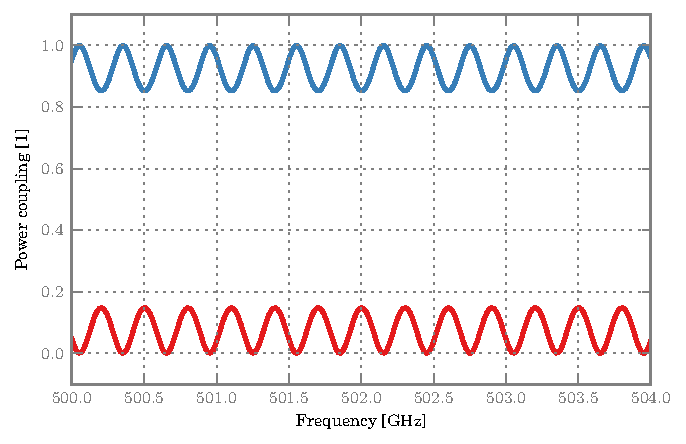
\includegraphics{simple_cavity_direct}
    \caption{Simple cavity, model result.}
    \caption*{
        The blue curve, on top, corresponds to the power coupling of port~6,
        that is the transmission through the cavity.
        The red curve, on the bottom, corresponds to the power coupling of port~1,
        that is the reflection on the cavity.
    }
    \label{fig:simple_cavity_direct}
\end{figure}
\begin{figure}[hbtp]
    \centering
    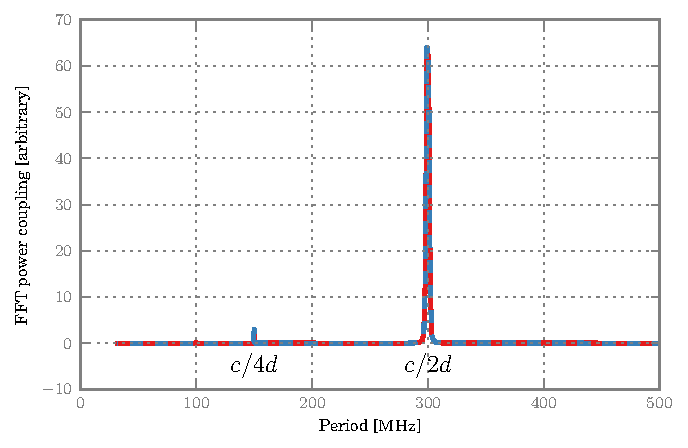
\includegraphics{simple_cavity_fft}
    \caption{Simple cavity, Fourier transform of the model result.}
    \caption*{
        The transmitted (blue) and reflected (red) wave show the same amount of modulation
        introduced by the cavity.
        The fundamental is at a period $F=c/2d$ with $c$ the speed of light in the cavity
        and $d$ the length of the cavity.
        An harmonic shows at $F=c/4d$,
        proving that the modulation is not perfectly sinusoidal.
        This spectrum was obtained by running the model for 4001 frequencies
        over a~\SI{64}{\giga\hertz} range,
        multiplying the result by a hanning window and taking a fast Fourier transform.
    }
    \label{fig:simple_cavity_fft}
\end{figure}

\Cref{fig:simple_cavity_direct} presents the result of the model for the following parameters:
\begin{itemize}
    \item refractive index $n_1=1.5$,
    \item refractive index $n_2=1.0$,
    \item distance between the interfaces $d=\SI{0.5}{\meter}$,
    \item frequency $f$ from \SIrange{500}{504}{\giga\hertz}.
\end{itemize}
The scattering matrices of the interfaces are derived from~\vref{eq:s_interface_normal} using $n_1$ and $n_2$.
The scattering matrix of the space between the interfaces is derived from~\vref{eq:scattering_distance} using $d$, $n_1$ and $f$.



%-----------------------------------------------------------------------------

\subsubsection{Periodicity}
According to \cref{eq:cavity_period}, we expect a periodicity of $F=c/2d$ where $c=c_0/n$ is the speed of light in the cavity and $d$ the length of the cavity.
With $c_0\approx \SI{2.998e8}{\meter\per\second}$, $n=1$ and $d=\SI{0.5}{\meter}$, we get $F \approx \SI{299.8}{\mega\hertz}$.

Our model agrees with our expectation, as shown by the fourrier transform in \cref{fig:simple_cavity_fft}.



%-----------------------------------------------------------------------------

\subsubsection{Energy conservation}
Examination of the results displayed in \cref{fig:simple_cavity_direct} reveals that energy is neither created nor destroyed.
The power is always positive, and the sum of the transmitted (blue) and reflected (red) power always equal 1 within numerical noise.
The power that is not transmitted through the cavity is reflected back to the source.



%=============================================================================

\subsection{Thin film beam splitter}

A thin dielectric film can be used as a beam splitter, as illustrated in \cref{fig:beam_splitter_principle}.
\begin{figure}[hbtp]
    \centering
    \input{beam_splitter_principle.pdf_tex}
    \caption{Beam splitter, principle.}
    \label{fig:beam_splitter_principle}
\end{figure}

This setup is one of the simplest way to inject local oscillator (LO) and sky signal together on a mixer.
What we have here is a heterodyne telescope.
The very transparent thin film couples most of the sky signal to the mixer, while coupling almost none of the local oscillator noise.
Unfortunately, the thin film is also transparent to the LO signal (narrow line at the LO frequency) required to pump the mixer, so the LO signal must be very strong.
This design wastes most of the LO power but has the advantage of being simple.
HIFI uses a similar approach for its bands 1, 2 and 3 (with wire grid polarizers instead of thin films though).

%-----------------------------------------------------------------------------

\subsubsection{Modeling the networks}

We can model the thin film using the principle described in \cref{sec:thin_film_at_oblique_incidence}.
Let us model a thin film of biaxially-oriented polyethylene terephthalate or ``boPET'', more commonly known under trade-mame ``Mylar''.
The table entry for ``PETP'' in the article of \citeauthor{lamb1996miscellaneous}~\cite{lamb1996miscellaneous} suggests that we choose 1.83 for the refractive index of the film at~\SI{500}{\giga\hertz}.
Using the notations of the article,
this 1.83 corresponds to the real part~$n$ of the refractive index~$\hat{n}=n-ik$.
The imaginary part~$k$ is given by the ``$\tan \delta$'' column of the table and
the equation (6) of that article, which links $\tan \delta$ to $k$: $\tan \delta = 2k/n$.
Therefore, $k = (n \tan \delta) / 2$.
With $n=1.83$ and $\tan \delta = 0.020$, we have $k=0.018$.
Our own conventions (deriving from~\cref{eq:e_z_t_real_minus}) require a sign flip: as explained in \vref{sec:polar_complex_notation}, a positive imaginary part creates absorption.
The complex refractive index of our thin film is $1.83+0.018i$.

% I know that the imaginary part of the refractive index corresponds to an absorption/gain.  The plus or minus sign probably depends on the convention chosen for k and omega.
% I have
% E = E_0 exp(ikz)
% k = \tau / \lambda
% \lambda = c / f
% c = c_0 / n
% k = \tau f n / c_0 = K n
% n = nr + i ni
% exp(iKnz) = exp(i K nr z - K ni z) = exp(iKnrz) exp(-Kniz)
% The greater ni, the stronger the attenuation.
% Therefore, I must keep ni positive.

To model the local oscillator and the mixer, I use networks that reflect \SI{10}{\percent} and transmit \SI{90}{\percent} of the incoming signal.
This is a very simplified model for a mixer or a local oscillator, but it does take into account their principle characteristic from a standing wave point of view: they reflect.

The two absorbers do not need any modeling: it is sufficient to leave the two corresponding ports of the thin film open.

%-----------------------------------------------------------------------------

\subsubsection{Simulation}
\begin{figure}[hbtp]
    \centering
    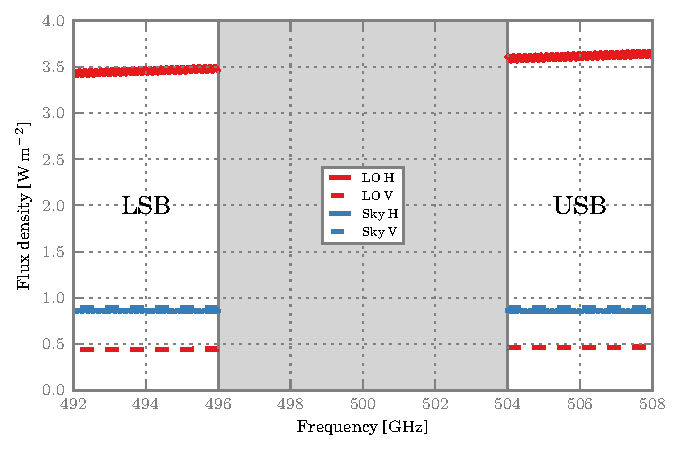
\includegraphics{thin_film_beam_splitter_detailed}
    \caption{Thin film beam splitter, detailed.}
    \label{fig:thin_film_beam_splitter_detailed}
\end{figure}
In the lower and upper side bands, the mixer receives power from two sources: the astronomical signal from the sky and the noise of the local oscillator.
In the case of HIFI, the local oscillator noise is typically two orders of magnitude stronger than the astronomical signal.
We arbitrarily set the power density from the sky at \SI{1}{\watt\per\meter\squared} and that of the local oscillator to \SI{100}{\watt\per\meter\squared}.
Since these two sources are not phase locked, we solve the system for each of them independantly.
The result is given on \cref{fig:thin_film_beam_splitter_detailed}.

We notice that the power of both the local oscillator signal and the sky signal have the same order of magnitude when hitting the mixer.
This is due to the fact that the thin film is mostly transparent, hardly reflective.
Because the sky is seen in transmission, its power is still very close to its emitted value of \SI{1}{\watt\per\meter\squared}, we couple most of the sky.
And because the local oscillator is seen in reflection, we couple only a small fraction of it (\SI{0.5}{\percent} or \SI{3.5}{\percent} depending on the polarization).
This increases the signal-to-noise ratio to an acceptable level.

The figure also illustrates that this beam splitter transmits V more than it transmits H.
As a result, V shows more sky power and less LO power.
It is in the interest of the astronomer to reject the horizontal polarization.
This can be done with a wire-grid polarizer or by using rectangular horns.

When examined closely, the H curves show some fast oscillations.
The V curves are also affected, as the next figure will show.
These oscillations are due to the cavity formed by the mixer and the local oscillator.
That cavity consists of $d=\SI{1}{\meter}$ or vacuum, which results in a period of $c_0 / 2d \approx \SI{150}{MHz}$.

The red curves show a slope.
The higher the frequency, the more LO power the mixer sees.
This slope is actually a portion of a very slow standing wave pattern.
It corresponds to the cavity formed by the two interfaces of the thin film itself.
With a speed of light of $c_0 / 1.83$ and a thickness of \SI{10}{\micro\meter}, we expect a standing wave pattern with a period of about \SI{8}{\tera\hertz}.
Calculating the real period involves knowing the pathlength of the beam inside the film, which requires some trigonometry, but the order remains at several terahertz.

In a real system, we would not have access to all the details of \cref{fig:thin_film_beam_splitter_detailed}.
Indeed, for a given frequency, we receive the sum of the LO and sky power without being able to tell them apart.
Furthermore, mixers fold spectra, which adds the lower and upper side bands together.
Finally, the polarizations become undistinguishable.
In \cref{fig:thin_film_beam_splitter_folded}, we have summed the two sources and folded the spectra; however we kept the polarization intact.
These summations were done in power and not in field, because the LSB, USB, LO and sky power are not phase locked to each other: each signal is coherent with itself only, not with the others.

\begin{figure}[hbtp]
    \centering
    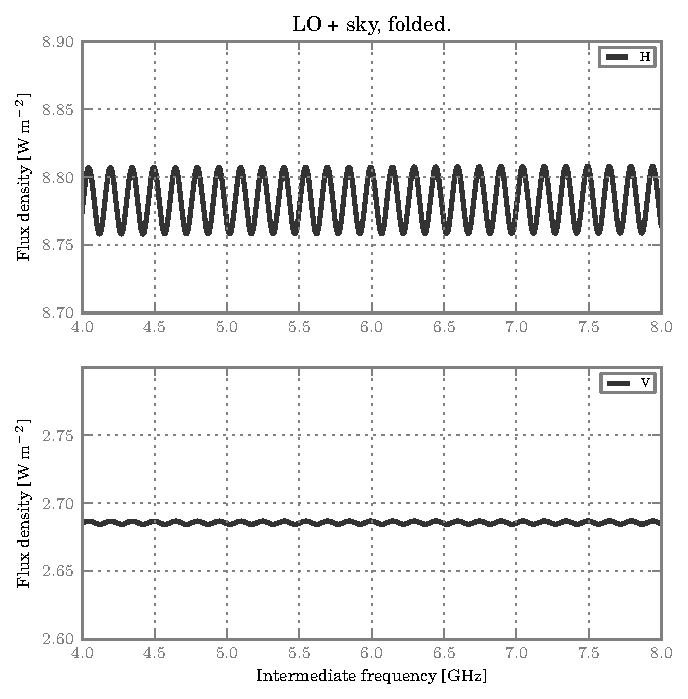
\includegraphics{thin_film_beam_splitter_folded}
    \caption{Thin film beam splitter, folded.}
    \label{fig:thin_film_beam_splitter_folded}
\end{figure}

The slope due to the cavity inside the thin film seems to have disappeared.
This is expected: the lower sideband is flipped before being added to the upper sideband.
Therefore, when the slope goes up for one, it goes down for the other,
and they compensate quite well.
Some other values for the LO frequency or film thickness can allow the thin film cavity to leave a more obvious signature on the folded spectrum.

This figure reveals that the V polarization is also affected by standing wave, as we mentionned earlier.
It is much weaker in V than in H because the thin film is more transparent for V.
This means that the V-polarized light is more likely to exit the cavity either toward the sky or toward the open port on the right, both perfect aborbers.
This standing wave pattern has a period of \SI{150}{\mega\hertz}, which is expected of the LO--mixer cavity.

\subsubsection{Sideband ratio}
Standing waves change the coupling of the mixer to the signal.
This coupling is a priori different in the lower and upper sideband.
Therefore, each channel of a folded spectrum is a priori imbalanced, giving more weight to either sideband.

In the HIFI consortium, we agreed on the following definition~\eqref{eq:sideband_ratio} of the sideband ratio as a metric for the imbalance between the two sidebands.
A perfectly balanced system has a sideband ratio of 0.5.
If the sideband ratio is greater than 0.5, then the channel is USB-dominated.
If it is lower than 0.5, the channel is LSB-dominated.
\begin{equation}
    \text{sideband ratio} =
    \frac{
        \text{USB power coupling}
    }{
        \text{LSB power coupling} + \text{USB power coupling}
    }
    \label{eq:sideband_ratio}
\end{equation}

\begin{figure}[hbtp]
    \centering
    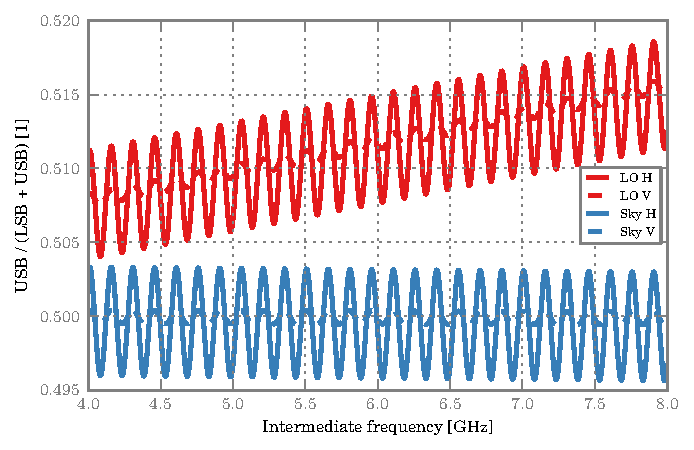
\includegraphics{thin_film_beam_splitter_sbr}
    \caption{Thin film beam splitter, sideband ratio.}
    \label{fig:thin_film_beam_splitter_sbr}
\end{figure}
\Cref{fig:thin_film_beam_splitter_sbr} shows the sideband ratio for the LO and the sky for both polarizations.
The slope comes from very slow modulation due to the cavity inside the thin film.
Note that it is clearly visible here, even on the sky, while it was hardly noticeable on the folded spectrum of \cref{fig:thin_film_beam_splitter_folded}.
A flat continuum does not guarantee a flat sideband ratio.

With this system, the standard deviation of the sideband ratio for is \SI{2.6}{\percent} for H and \SI{0.3}{\percent} for V.
This is the error that we can expect when measuring a thin emission line on a perfectly flat continuum after an infinitely long integration time: the line can fall anywhere between a peak and a crest of this standing wave pattern.

\subsubsection{The many LO--mixer cavities}

\Cref{fig:thin_film_beam_splitter_folded_fft} shows
the fast Fourier Transform of \cref{fig:thin_film_beam_splitter_folded} (using a Hanning window).
It peaks at the expected~\SI{150}{\mega\hertz} and shows a very weak harmonic at~\SI{75}{\mega\hertz}.
The harmonics are very weak because the cavity is of very low quality: the film is very transparent and the light leaves the cavity quickly.

\begin{figure}[hbtp]
    \centering
    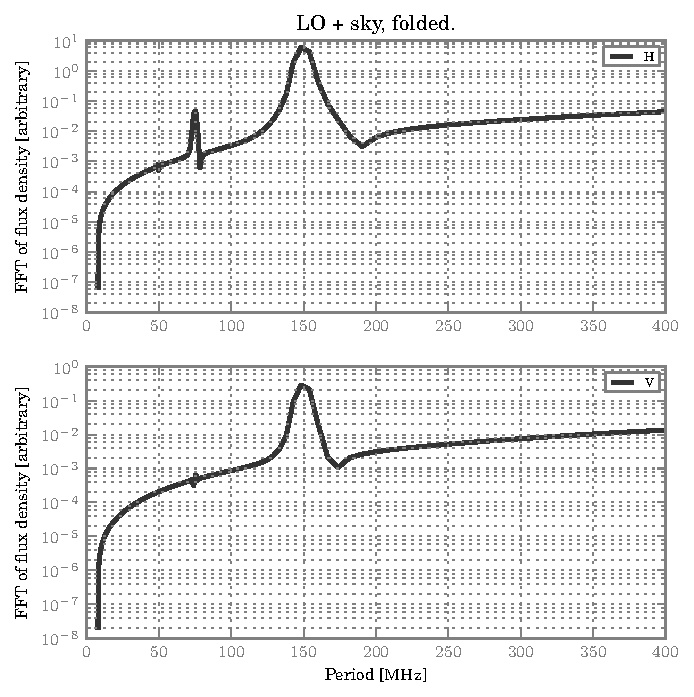
\includegraphics{thin_film_beam_splitter_folded_fft}
    \caption{Thin film beam splitter, folded, FFT.}
    \label{fig:thin_film_beam_splitter_folded_fft}
\end{figure}

The astute reader may be wondering why we are observing only two cavities (LO--mixer and inside thin film) instead of an infinity.
Indeed, there is no such thing as \textit{the} LO--mixer cavity, there are an infinity of them.
The shortest one is the one corresponding to a single reflection on the near side of the thin film.
Then, another possible path involves entering the thin film, being reflected by the far side, traversing the film again, and being transmitted toward the detector.
A third path involves two round-trips inside the film, and a fourth path involves three round-trips, etc.
Why don't these many cavities show up as as many peaks on the FFT?
The answer is simple: our FFT does not have enough resolution.

Our bandpass $B$ of \SI{4}{\giga\hertz} does not allow to resolve a variation of \SI{10}{\micro\meter} in a cavity.
$B = c / 2d$ with $d=\SI{10}{\micro\meter}$ and $c=c_0$ yields $B \approx \SI{15}{\tera\hertz}$, which is way beyond our \SI{4}{\giga\hertz}.
If we reverse the calculation, $d=c/2B$ for $B=\SI{4}{\giga\hertz}$ gives $d \approx \SI{37}{mm}$: our FFT can distinguish cavities that differ by more than \SI{4}{\centi\meter}.
This limitation affects only the FFT as a tool used for visualizing our data; our model has no such limitation.

\begin{figure}[hbtp]
    \centering
    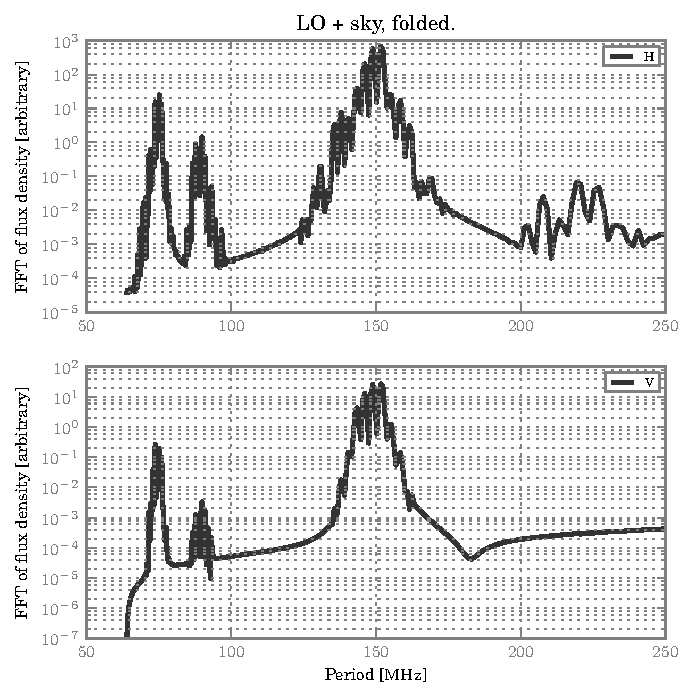
\includegraphics{thin_film_beam_splitter_folded_fft_hr}
    \caption{Thin film beam splitter, folded, FFT, high resolution.}
    \label{fig:thin_film_beam_splitter_folded_fft_hr}
\end{figure}
\Cref{fig:thin_film_beam_splitter_folded_fft_hr} shows the FFT of the same system for a bandwidth of~\SI{32}{\giga\hertz}, a film thickness of~\SI{1}{\centi\meter}, and no imaginary part in the refractive index of the mylar (otherwise the absorption would hide the result).
Once the system is modified to meet the expectations of the FFT, then the FFT does show the expected many peaks around~\SI{150}{\mega\hertz}, which prove that our model takes into account the infinity of LO--mixer cavities.



\section{Conclusion}
%In the best case scenario, we will manage to figure out all the physical parameters of HIFI, allowing us to recalibrate the entire data archive of HIFI to cancel the effect of interferences.
%Naturally, this best case scenario is somewhat ambitious: obtaining a perfect quantitative match between the model and the data is a difficult task.

%More realistically, the model that we propose could become very helpful to the engineers who are designing instruments.
%Our technique can give useful qualitative predictions, even when the parameters of the models are nothing but educated guesses (more on this in~\cref{sec:chapter3})
%Like good software developers do not optimize their code until profiling indicates which routines are bottlenecks, good engineers do not spend resources trying to reduce interferences unless they know which ones matter and where they occur.
